\chapter{Simultaneous size and density determination of polymeric colloids}
\label{chap:simultaneous_size_density}
The current advances in nanomaterial development for medical applications are focused towards tailoring polymeric nano-drug carriers with flexible surface functionalisation and controlled morphologies\citep{euliss_imparting_2006,yang_shape-memory_2005}. Size and shape, combined with the choice of polymer and the mechanical properties, are fundamental and defining aspects of the particle functions, e.g. their \emph{in-vivo} biodistribution\citep{vittaz_effect_1996,mitragotri_physical_2009,doshi_designer_2009} or their drug-delivery efficacy\citep{powers_research_2006}. Therefore, a full and consistent characterisation of all properties of nanoparticles is of crucial importance and must be carefully adressed, especially for polymeric NPs due to their typical complicate internal structure.

This work demonstrates the simultaneous size and density determination using continuous contrast variation technique in SAXS with 3 polymeric particles of different sizes and polymeric species. By means of an aqueous sucrose density gradient, the measurements were achieved along a large range of suspending medium densities, from water density to that of poly(methyl methacrylate)'s, highlighting the relevance of the technique across a wide spectrum of polymers.

This chapter discusses the applicability of this method for the traceable size determination of these colloids, where a high-resolution size distribution of the particles is presented. Focusing on a low-density colloid, different evaluation approaches to SAXS contrast variation experiments are discussed and the advantages and drawbacks of a model-free formulation like the isoscattering point position are discussed, together with the accuracy of the scattering shape factor. In addition, a form factor model is fitted to the scattering curves to obtain decisive information about the internal morphology of the particle, which is not directly available by other techniques such as transmission scanning electron microscopy (TSEM), differential centrifugal sedimentation (DCS)\citep{fielding_correcting_2012} or atomic force microscopy (AFM). 

Besides, the ability of this technique to determine the density of polymeric colloids in suspension is also discussed. Normally, the density of the suspended particles can not be compared to the bulk density of the dry material. Such a complex question has been adressed by different methods, though with evident limitations. For example, the density of polymeric beads has been measured previously with field-flow fractionation (FFF) with high-accuracy but at the expense of \emph{a priori} assumptions about the morphology of the particle\citep{giddings_density_1981,yang_colloid_1983,caldwell_measurement_1986}. Assuming the Stokes' diameter as the actual size of the colloid, recent advances in analytical ultracentrifugation allow the complementary characterisation of the size, density and molecular weight of gold nanoparticles\citep{carney_determination_2011}.

The density of the 3 polymeric colloids was also analysed by DCS and the results compared and discussed with those obtained by SAXS. DCS uses the sedimentation of particles through a density gradient to measure high resolution particle size distributions\citep{minelli_characterization_2014}. Its accuracy typically depends on the knowledge of the density of the particles. When the size of the particle is known, DCS can alternatively be used to measure average particle's density.

In this study, the size and density of low-density particles is independently determined by performing DCS measurements with two different discs using the sedimentation and flotation respectively of the particles through a density gradient and solving the relative Stokes' equations. A similar approach to DCS which combines the results of two independent measurements has been investigated previously. For example, \cite{neumann_new_2013} used two sucrose gradients resulting in different viscosities and densities, where the altered settling velocity combined with linear regression analysis was used for the calculation of the size and density of silica nanoparticles and viruses. \cite{bell_emerging_2012} adopted a two gradient method based on the variation of the sucrose concentration to determine the density of the St\"ober silica and the calibration standards used in DCS.

\section{Materials and methods}
In this section, a detailed description of the polymeric nanoparticles employed in the experiments is presented. The experimental procedure of the continuous contrast variation technique is thoroughly discussed already in chapter \ref{chap:density_gradient_SAXS}, thus the focus of the section lies only on the DCS technique. Special interest is put on the description of the combined DCS approach based on the floating-sedimentation principle.


\subsection{Polymeric particles}

The experiments were performed using 3 different types of polymeric nanoparticles, whose sizes range from 100 nm to around 187 nm. Carboxylated poly(methyl methacrylate) colloids (PMMA-COOH) with a nominal diameter of 187 nm and plain polystyrene particles (PS-Plain) polymerized with $<1$ wt$\%$ of a surface-active co-monomer with a nominal diameter of 147 nm were purchased from Microparticles (Berlin, \emph{Germany}). The PS-COOH particles are described in detail in chapter \ref{chap:density_gradient_SAXS} and are composed of a PS core surrounded by a PMMA shell. The phyisical densities of the NPs range from that of PS (1.05 g cm$^{-3}$) until PMMA's, which has a density of ca. 1.18 g cm$^{-3}$.

For the preparation of the high density aqueous sucrose solutions employed in the density gradient capillaries, the suspended colloids were mixed with a sucrose mass fraction of 21.2 $\%$, 42.5 $\%$ and 13.4 $\%$ for the PS-COOH, PMMA-COOH and PS-Plain particles respectively.


\subsection{Differential Centrifuge Sedimentation (DCS)}
\label{sec:DCS_experimental}
DCS measurements were performed with a CPS DC20000 instrument (CPS Instruments, Prairieville, LA, \emph{USA}) upgraded to DC24000 for the PS-Plain measurements. The radial position of the detector was measured by injecting 100 $\mu$L aliquots of water into the spinning disc initially empty until the accumulation of water produced a response in the detector. For the density gradient formation, the disc was filled with 14.4 mL of a sucrose (Amresco LLC, OH, \emph{USA}) solution topped with 0.5 mL of dodecane to prevent evaporation. The detailed information of the gradients is summarised in table \ref{tab:DCSParameters}. Measurements of PS-COOH and PMMA-COOH at 0.05 \% w/v concentration were performed in triplicate. PS-Plain measurements were repeated seven times for each setup. Injection volumes were 100 $\mu$L. 

\begin{table*}[]
\centering
\caption{Parameters of the different DCS setups: composition of the sucrose gradients, average density of the gradients $\rho_f$, angular speed of the centrifuge $\Omega$ and type of calibrant.}
\label{tab:DCSParameters}
\begin{tabular}{l|c|c|c|c|}
\cline{2-5}
\multicolumn{1}{c|}{}                         & Sucrose concentration (w/w)    & $\rho_f$ (g cm$^{-3}$) & $\Omega$ (rpm)  & Calibrant \\ \hline
\multicolumn{1}{|l|}{PS-COOH}    & from 2 \% to 8 \% in H$_2$0  & 1.013                  & 2.0$\cdot 10^4$                  & A         \\ \hline
\multicolumn{1}{|l|}{PMMA-COOH}  & from 4 \% to 12 \% in H$_2$0 & 1.025                  & 2.0$\cdot 10^4$                  & B         \\ \hline
\multicolumn{1}{|l|}{PS-Plain}      & from 2 \% to 8 \% in H$_2$0  & 1.013     & 2.4$\cdot 10^4$                  & B        \\ \hline
\multicolumn{1}{|l|}{PS-Plain*} & from 4 \% to 12 \% in D$_2$0 & 1.140     & 2.4$\cdot 10^4$                  & C         \\ \hline

\end{tabular}\\[0.3\baselineskip]
\begin{minipage}{15cm}
	\begin{raggedright}
	*\small{Low density disc}
	\end{raggedright}
\end{minipage}
\label{tab:composition}
\end{table*}

The measured turbidity at 405 nm was converted to the number of particles for each measured diameter by treating the particles as spherical Mie scatterers with no optical absorbance at the incident wavelength. Three different types of calibration particles were used: poly(vinyl chloride) colloids in water with density of 1.385 g cm$^{-3}$ and nominal size of $(223\pm5)$ nm (calibrant A) and $(239\pm5)$ nm (calibrant B) and polybutadiene colloids in 16 \% sucrose mass fraction in heavy water with nominal size of $(510\pm20)$ nm and density of 0.91 g cm$^{-3}$ (calibrant C). 

A standard disc configuration where the particles sediment through a lower density gradient was used and additionally, a more recently developed set up which makes use of a disc where colloids float through a higher density gradient was also used for PS-Plain due to their low density\citep{fitzpatrick_structure_1998}. Typically, the DCS diameter $D_p$ or density $\rho_p$ of a spherical particle is derived from the Stokes' law:

\begin{equation}
D_p=\sqrt{\frac{18\eta\ln\sfrac{R_f}{R_i}}{\left( \rho_p - \rho_{\text{fluid}} \right)\omega^2 t_p}}
\label{eq:stokes}
\end{equation}

where $t_p$ is the sedimentation time between radii of rotation $R_f$ and $R_i$ of the particle, $\eta$ and $\rho_f$ are the viscosity and the density of the fluid respectively and $\omega$ is the disc angular frequency. If a calibrant of known size $D_c$ and density $\rho_c$ is measured with the same set up, the investigated particle diameter can be expressed as:

\begin{equation}
D_p=D_c\sqrt{\frac{\left( \rho_c - \rho_{\text{fluid}} \right) t_c}{\left( \rho_p - \rho_{\text{fluid}} \right) t_p}}
\label{eq:software}
\end{equation}

By using the combination of DCS measurements performed in two different fluids, one with density $\rho_L$ and one with higher density $\rho_H$, the values of $D_p$ and $\rho_p$ can be independently found by solving analytically the following system of equations:

\begin{equation}
\bm{D_p} = D_{cH}\sqrt{\frac{\left( \rho_{cH} - \rho_H \right) t_{cH}}{\left( \bm{\rho_p} - \rho_H \right) t_{pH}}} = D_{cL}\sqrt{\frac{\left( \rho_{cL} - \rho_L \right) t_{cL}}{\left( \bm{\rho_p} - \rho_L \right) t_{pL}}}
\label{eq:DCS_sys}
\end{equation}

where $cH$ and $cL$ denote the calibrants used with high and low density fluids respectively and $t_{pH}$ and $t_{pL}$ are the sedimentation times of the particles measured in the high and low density fluids respectively. The measurement uncertanties given in the text include both statistical and systematic uncertainty propagated from Stokes' equations.

\section{Determination of the particle size distribution}
\label{sec:size_validation}

\begin{figure}
	\begin{center}
		% GNUPLOT: LaTeX picture with Postscript
\begingroup
  \makeatletter
  \providecommand\color[2][]{%
    \GenericError{(gnuplot) \space\space\space\@spaces}{%
      Package color not loaded in conjunction with
      terminal option `colourtext'%
    }{See the gnuplot documentation for explanation.%
    }{Either use 'blacktext' in gnuplot or load the package
      color.sty in LaTeX.}%
    \renewcommand\color[2][]{}%
  }%
  \providecommand\includegraphics[2][]{%
    \GenericError{(gnuplot) \space\space\space\@spaces}{%
      Package graphicx or graphics not loaded%
    }{See the gnuplot documentation for explanation.%
    }{The gnuplot epslatex terminal needs graphicx.sty or graphics.sty.}%
    \renewcommand\includegraphics[2][]{}%
  }%
  \providecommand\rotatebox[2]{#2}%
  \@ifundefined{ifGPcolor}{%
    \newif\ifGPcolor
    \GPcolortrue
  }{}%
  \@ifundefined{ifGPblacktext}{%
    \newif\ifGPblacktext
    \GPblacktextfalse
  }{}%
  % define a \g@addto@macro without @ in the name:
  \let\gplgaddtomacro\g@addto@macro
  % define empty templates for all commands taking text:
  \gdef\gplbacktext{}%
  \gdef\gplfronttext{}%
  \makeatother
  \ifGPblacktext
    % no textcolor at all
    \def\colorrgb#1{}%
    \def\colorgray#1{}%
  \else
    % gray or color?
    \ifGPcolor
      \def\colorrgb#1{\color[rgb]{#1}}%
      \def\colorgray#1{\color[gray]{#1}}%
      \expandafter\def\csname LTw\endcsname{\color{white}}%
      \expandafter\def\csname LTb\endcsname{\color{black}}%
      \expandafter\def\csname LTa\endcsname{\color{black}}%
      \expandafter\def\csname LT0\endcsname{\color[rgb]{1,0,0}}%
      \expandafter\def\csname LT1\endcsname{\color[rgb]{0,1,0}}%
      \expandafter\def\csname LT2\endcsname{\color[rgb]{0,0,1}}%
      \expandafter\def\csname LT3\endcsname{\color[rgb]{1,0,1}}%
      \expandafter\def\csname LT4\endcsname{\color[rgb]{0,1,1}}%
      \expandafter\def\csname LT5\endcsname{\color[rgb]{1,1,0}}%
      \expandafter\def\csname LT6\endcsname{\color[rgb]{0,0,0}}%
      \expandafter\def\csname LT7\endcsname{\color[rgb]{1,0.3,0}}%
      \expandafter\def\csname LT8\endcsname{\color[rgb]{0.5,0.5,0.5}}%
    \else
      % gray
      \def\colorrgb#1{\color{black}}%
      \def\colorgray#1{\color[gray]{#1}}%
      \expandafter\def\csname LTw\endcsname{\color{white}}%
      \expandafter\def\csname LTb\endcsname{\color{black}}%
      \expandafter\def\csname LTa\endcsname{\color{black}}%
      \expandafter\def\csname LT0\endcsname{\color{black}}%
      \expandafter\def\csname LT1\endcsname{\color{black}}%
      \expandafter\def\csname LT2\endcsname{\color{black}}%
      \expandafter\def\csname LT3\endcsname{\color{black}}%
      \expandafter\def\csname LT4\endcsname{\color{black}}%
      \expandafter\def\csname LT5\endcsname{\color{black}}%
      \expandafter\def\csname LT6\endcsname{\color{black}}%
      \expandafter\def\csname LT7\endcsname{\color{black}}%
      \expandafter\def\csname LT8\endcsname{\color{black}}%
    \fi
  \fi
  \setlength{\unitlength}{0.0500bp}%
  \begin{picture}(5668.00,4534.00)%
    \gplgaddtomacro\gplbacktext{%
      \csname LTb\endcsname%
      \put(990,704){\makebox(0,0)[r]{\strut{} 0.1}}%
      \csname LTb\endcsname%
      \put(990,1355){\makebox(0,0)[r]{\strut{} 1}}%
      \csname LTb\endcsname%
      \put(990,2006){\makebox(0,0)[r]{\strut{} 10}}%
      \csname LTb\endcsname%
      \put(990,2657){\makebox(0,0)[r]{\strut{} 100}}%
      \csname LTb\endcsname%
      \put(990,3308){\makebox(0,0)[r]{\strut{} 1000}}%
      \csname LTb\endcsname%
      \put(990,3958){\makebox(0,0)[r]{\strut{} 10000}}%
      \csname LTb\endcsname%
      \put(1122,484){\makebox(0,0){\strut{} 0.02}}%
      \csname LTb\endcsname%
      \put(1586,484){\makebox(0,0){\strut{} 0.03}}%
      \csname LTb\endcsname%
      \put(2171,484){\makebox(0,0){\strut{} 0.05}}%
      \csname LTb\endcsname%
      \put(2964,484){\makebox(0,0){\strut{} 0.1}}%
      \csname LTb\endcsname%
      \put(3758,484){\makebox(0,0){\strut{} 0.2}}%
      \csname LTb\endcsname%
      \put(4222,484){\makebox(0,0){\strut{} 0.3}}%
      \csname LTb\endcsname%
      \put(4807,484){\makebox(0,0){\strut{} 0.5}}%
      \put(220,2486){\rotatebox{-270}{\makebox(0,0){\strut{}Scattering Intensity / a.u.}}}%
      \put(3196,154){\makebox(0,0){\strut{}$q$ / nm$^{-1}$}}%
    }%
    \gplgaddtomacro\gplfronttext{%
      \csname LTb\endcsname%
      \put(3063,1386){\makebox(0,0)[r]{\strut{}PS-Plain in buffer}}%
      \csname LTb\endcsname%
      \put(3063,1056){\makebox(0,0)[r]{\strut{}Core-Shell Fit}}%
    }%
    \gplgaddtomacro\gplbacktext{%
      \csname LTb\endcsname%
      \put(3862,3016){\makebox(0,0)[r]{\strut{}\footnotesize 333}}%
      \csname LTb\endcsname%
      \put(3862,3278){\makebox(0,0)[r]{\strut{}\footnotesize 337}}%
      \csname LTb\endcsname%
      \put(3862,3539){\makebox(0,0)[r]{\strut{}\footnotesize 341}}%
      \csname LTb\endcsname%
      \put(3862,3801){\makebox(0,0)[r]{\strut{}\footnotesize 345}}%
      \csname LTb\endcsname%
      \put(3994,2796){\makebox(0,0){\strut{}\footnotesize 0}}%
      \csname LTb\endcsname%
      \put(4367,2796){\makebox(0,0){\strut{}\footnotesize 25}}%
      \csname LTb\endcsname%
      \put(4740,2796){\makebox(0,0){\strut{}\footnotesize 50}}%
      \csname LTb\endcsname%
      \put(5112,2796){\makebox(0,0){\strut{}\footnotesize 75}}%
      \put(3356,3572){\rotatebox{-270}{\makebox(0,0){\strut{}\footnotesize{$\rho_e$ / nm$^{-3}$}}}}%
      \put(4575,2466){\makebox(0,0){\strut{}\footnotesize{$R$} / nm}}%
    }%
    \gplgaddtomacro\gplfronttext{%
    }%
    \gplbacktext
    \put(0,0){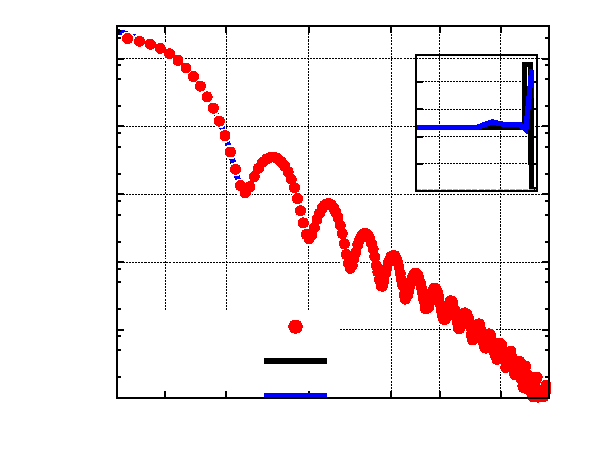
\includegraphics{PSPlainSingleContrastSAXS}}%
    \gplfronttext
  \end{picture}%
\endgroup

	\end{center}
	\caption{Scattering curve of PS-Plain in buffer: A core–shell and onion model fit to the experimental scattering curve are presented. In the inset, the electron density radial profile
	\label{fig:PSPlainSingleContrastSAXS}
of these fits is shown, assuming the core is polystyrene with a density of 339.7 nm$^{-3}$.}
\end{figure}

In figure \ref{fig:PSPlainSingleContrastSAXS}, the SAXS curve of the  PS-Plain particles in buffer at a single-contrast is shown. The large number of minima observed in the curve is remarkable and indicates the high monodispersity of the sample, which allows a traceable size determination of these colloids.

Upon trying different form factor fits detailed in section \ref{sec:SAXS_theory}, a simple core-shell structure with a sharp interface (eq. \ref{eq:ff_cs}) was found to be the most suitable, suggesting a heterogeneous structure which is eluded by other characterization techniques, e.g. microscopy. The obtained particle diameter was $(147.0\pm4.7)$ nm, where the fit uncertainty was calculated with a confidence level of one standard deviation ($k=1$) by examining the change in $\chi^2$ when varying the diameter. The radial electron density profile of the core-shell fit is shown in the inset of figure \ref{fig:PSPlainSingleContrastSAXS}, where a thin shell with high density surrounds a lighter core. This structure is likely due to the non-reacted monomers in the main matrix or the highly hydrophilic behaviour of the co-monomer, segregating polystyrene to the core.

In figure \ref{fig:PSPlainSingleContrastSAXS}, it is also depicted the fit of the form factor \ref{eq:multicore-shell} with 7 shells with a linear electron density gradient. This fit is in very good agreement with the experimental data as well and presents a $\chi^2$ value 20 times lower than the compact spheres model fit. Although the radial electron density profile shown in the inset coincides qualitatively with the core-shell model, the result might ot be unique due to the large number of fiting parameters (14) and care must be taken.

The PS-Plain morphology was further studied using the density gradient contrast variation technique described in chapter \ref{chap:density_gradient_SAXS} by varying the suspending medium electron density from 333.2 to 350.2 nm$^{-3}$. By increasing the solvent contrast, the changes of the features in the scattering curves presented in figure \ref{fig:PSPlainContinuousSAXS} and the appearance of isoscattering points prove the multi-component composition of this colloid.

\begin{figure}%[htbp]
	\centering
		\subfloat[Scattering curves]{\resizebox{0.44\linewidth}{!}{% GNUPLOT: LaTeX picture with Postscript
\begingroup
  \makeatletter
  \providecommand\color[2][]{%
    \GenericError{(gnuplot) \space\space\space\@spaces}{%
      Package color not loaded in conjunction with
      terminal option `colourtext'%
    }{See the gnuplot documentation for explanation.%
    }{Either use 'blacktext' in gnuplot or load the package
      color.sty in LaTeX.}%
    \renewcommand\color[2][]{}%
  }%
  \providecommand\includegraphics[2][]{%
    \GenericError{(gnuplot) \space\space\space\@spaces}{%
      Package graphicx or graphics not loaded%
    }{See the gnuplot documentation for explanation.%
    }{The gnuplot epslatex terminal needs graphicx.sty or graphics.sty.}%
    \renewcommand\includegraphics[2][]{}%
  }%
  \providecommand\rotatebox[2]{#2}%
  \@ifundefined{ifGPcolor}{%
    \newif\ifGPcolor
    \GPcolortrue
  }{}%
  \@ifundefined{ifGPblacktext}{%
    \newif\ifGPblacktext
    \GPblacktextfalse
  }{}%
  % define a \g@addto@macro without @ in the name:
  \let\gplgaddtomacro\g@addto@macro
  % define empty templates for all commands taking text:
  \gdef\gplbacktext{}%
  \gdef\gplfronttext{}%
  \makeatother
  \ifGPblacktext
    % no textcolor at all
    \def\colorrgb#1{}%
    \def\colorgray#1{}%
  \else
    % gray or color?
    \ifGPcolor
      \def\colorrgb#1{\color[rgb]{#1}}%
      \def\colorgray#1{\color[gray]{#1}}%
      \expandafter\def\csname LTw\endcsname{\color{white}}%
      \expandafter\def\csname LTb\endcsname{\color{black}}%
      \expandafter\def\csname LTa\endcsname{\color{black}}%
      \expandafter\def\csname LT0\endcsname{\color[rgb]{1,0,0}}%
      \expandafter\def\csname LT1\endcsname{\color[rgb]{0,1,0}}%
      \expandafter\def\csname LT2\endcsname{\color[rgb]{0,0,1}}%
      \expandafter\def\csname LT3\endcsname{\color[rgb]{1,0,1}}%
      \expandafter\def\csname LT4\endcsname{\color[rgb]{0,1,1}}%
      \expandafter\def\csname LT5\endcsname{\color[rgb]{1,1,0}}%
      \expandafter\def\csname LT6\endcsname{\color[rgb]{0,0,0}}%
      \expandafter\def\csname LT7\endcsname{\color[rgb]{1,0.3,0}}%
      \expandafter\def\csname LT8\endcsname{\color[rgb]{0.5,0.5,0.5}}%
    \else
      % gray
      \def\colorrgb#1{\color{black}}%
      \def\colorgray#1{\color[gray]{#1}}%
      \expandafter\def\csname LTw\endcsname{\color{white}}%
      \expandafter\def\csname LTb\endcsname{\color{black}}%
      \expandafter\def\csname LTa\endcsname{\color{black}}%
      \expandafter\def\csname LT0\endcsname{\color{black}}%
      \expandafter\def\csname LT1\endcsname{\color{black}}%
      \expandafter\def\csname LT2\endcsname{\color{black}}%
      \expandafter\def\csname LT3\endcsname{\color{black}}%
      \expandafter\def\csname LT4\endcsname{\color{black}}%
      \expandafter\def\csname LT5\endcsname{\color{black}}%
      \expandafter\def\csname LT6\endcsname{\color{black}}%
      \expandafter\def\csname LT7\endcsname{\color{black}}%
      \expandafter\def\csname LT8\endcsname{\color{black}}%
    \fi
  \fi
  \setlength{\unitlength}{0.0500bp}%
  \begin{picture}(5668.00,4534.00)%
    \gplgaddtomacro\gplbacktext{%
      \csname LTb\endcsname%
      \put(858,1156){\makebox(0,0)[r]{\strut{} 1}}%
      \csname LTb\endcsname%
      \put(858,2020){\makebox(0,0)[r]{\strut{} 10}}%
      \csname LTb\endcsname%
      \put(858,2884){\makebox(0,0)[r]{\strut{} 100}}%
      \csname LTb\endcsname%
      \put(858,3749){\makebox(0,0)[r]{\strut{} 1000}}%
      \csname LTb\endcsname%
      \put(1287,484){\makebox(0,0){\strut{} 0.03}}%
      \csname LTb\endcsname%
      \put(1858,484){\makebox(0,0){\strut{} 0.05}}%
      \csname LTb\endcsname%
      \put(2633,484){\makebox(0,0){\strut{} 0.1}}%
      \csname LTb\endcsname%
      \put(3408,484){\makebox(0,0){\strut{} 0.2}}%
      \csname LTb\endcsname%
      \put(3862,484){\makebox(0,0){\strut{} 0.3}}%
      \csname LTb\endcsname%
      \put(4433,484){\makebox(0,0){\strut{} 0.5}}%
      \put(220,2266){\rotatebox{-270}{\makebox(0,0){\strut{}Scattering Intensity / a.u.}}}%
      \put(2711,154){\makebox(0,0){\strut{}$q$ / nm$^{-1}$}}%
    }%
    \gplgaddtomacro\gplfronttext{%
      \csname LTb\endcsname%
      \put(4692,704){\makebox(0,0)[l]{\strut{}\fsmedium 334}}%
      \put(4692,1213){\makebox(0,0)[l]{\strut{}\fsmedium 336}}%
      \put(4692,1722){\makebox(0,0)[l]{\strut{}\fsmedium 338}}%
      \put(4692,2231){\makebox(0,0)[l]{\strut{}\fsmedium 340}}%
      \put(4692,2741){\makebox(0,0)[l]{\strut{}\fsmedium 342}}%
      \put(4692,3250){\makebox(0,0)[l]{\strut{}\fsmedium 344}}%
      \put(4692,3759){\makebox(0,0)[l]{\strut{}\fsmedium 346}}%
      \put(4692,4269){\makebox(0,0)[l]{\strut{}\fsmedium 348}}%
      \put(5418,2486){\rotatebox{-90}{\makebox(0,0){\strut{}\fsmedium Solvent Electron Density / nm$^{-3}$}}}%
    }%
    \gplbacktext
    \put(0,0){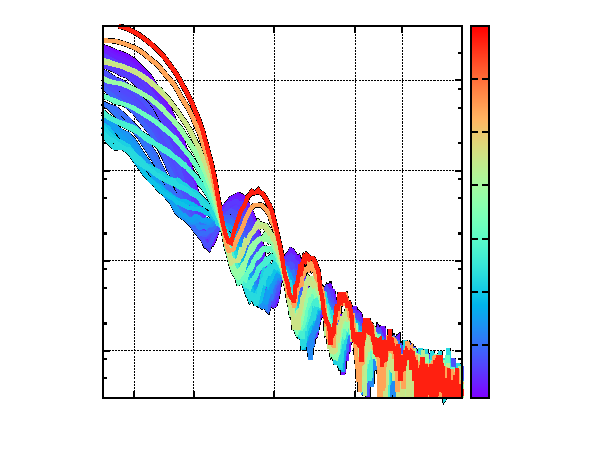
\includegraphics{PSPlainContinuousSAXS}}%
    \gplfronttext
  \end{picture}%
\endgroup
}\label{fig:PSPlainContinuousSAXS}}
		\subfloat[Isoscattering point positions]{\resizebox{0.44\linewidth}{!}{% GNUPLOT: LaTeX picture with Postscript
\begingroup
  \makeatletter
  \providecommand\color[2][]{%
    \GenericError{(gnuplot) \space\space\space\@spaces}{%
      Package color not loaded in conjunction with
      terminal option `colourtext'%
    }{See the gnuplot documentation for explanation.%
    }{Either use 'blacktext' in gnuplot or load the package
      color.sty in LaTeX.}%
    \renewcommand\color[2][]{}%
  }%
  \providecommand\includegraphics[2][]{%
    \GenericError{(gnuplot) \space\space\space\@spaces}{%
      Package graphicx or graphics not loaded%
    }{See the gnuplot documentation for explanation.%
    }{The gnuplot epslatex terminal needs graphicx.sty or graphics.sty.}%
    \renewcommand\includegraphics[2][]{}%
  }%
  \providecommand\rotatebox[2]{#2}%
  \@ifundefined{ifGPcolor}{%
    \newif\ifGPcolor
    \GPcolortrue
  }{}%
  \@ifundefined{ifGPblacktext}{%
    \newif\ifGPblacktext
    \GPblacktextfalse
  }{}%
  % define a \g@addto@macro without @ in the name:
  \let\gplgaddtomacro\g@addto@macro
  % define empty templates for all commands taking text:
  \gdef\gplbacktext{}%
  \gdef\gplfronttext{}%
  \makeatother
  \ifGPblacktext
    % no textcolor at all
    \def\colorrgb#1{}%
    \def\colorgray#1{}%
  \else
    % gray or color?
    \ifGPcolor
      \def\colorrgb#1{\color[rgb]{#1}}%
      \def\colorgray#1{\color[gray]{#1}}%
      \expandafter\def\csname LTw\endcsname{\color{white}}%
      \expandafter\def\csname LTb\endcsname{\color{black}}%
      \expandafter\def\csname LTa\endcsname{\color{black}}%
      \expandafter\def\csname LT0\endcsname{\color[rgb]{1,0,0}}%
      \expandafter\def\csname LT1\endcsname{\color[rgb]{0,1,0}}%
      \expandafter\def\csname LT2\endcsname{\color[rgb]{0,0,1}}%
      \expandafter\def\csname LT3\endcsname{\color[rgb]{1,0,1}}%
      \expandafter\def\csname LT4\endcsname{\color[rgb]{0,1,1}}%
      \expandafter\def\csname LT5\endcsname{\color[rgb]{1,1,0}}%
      \expandafter\def\csname LT6\endcsname{\color[rgb]{0,0,0}}%
      \expandafter\def\csname LT7\endcsname{\color[rgb]{1,0.3,0}}%
      \expandafter\def\csname LT8\endcsname{\color[rgb]{0.5,0.5,0.5}}%
    \else
      % gray
      \def\colorrgb#1{\color{black}}%
      \def\colorgray#1{\color[gray]{#1}}%
      \expandafter\def\csname LTw\endcsname{\color{white}}%
      \expandafter\def\csname LTb\endcsname{\color{black}}%
      \expandafter\def\csname LTa\endcsname{\color{black}}%
      \expandafter\def\csname LT0\endcsname{\color{black}}%
      \expandafter\def\csname LT1\endcsname{\color{black}}%
      \expandafter\def\csname LT2\endcsname{\color{black}}%
      \expandafter\def\csname LT3\endcsname{\color{black}}%
      \expandafter\def\csname LT4\endcsname{\color{black}}%
      \expandafter\def\csname LT5\endcsname{\color{black}}%
      \expandafter\def\csname LT6\endcsname{\color{black}}%
      \expandafter\def\csname LT7\endcsname{\color{black}}%
      \expandafter\def\csname LT8\endcsname{\color{black}}%
    \fi
  \fi
  \setlength{\unitlength}{0.0500bp}%
  \begin{picture}(5668.00,4534.00)%
    \gplgaddtomacro\gplbacktext{%
      \csname LTb\endcsname%
      \put(858,682){\makebox(0,0)[r]{\strut{} 0.02}}%
      \csname LTb\endcsname%
      \put(858,1493){\makebox(0,0)[r]{\strut{} 0.05}}%
      \csname LTb\endcsname%
      \put(858,2107){\makebox(0,0)[r]{\strut{} 0.1}}%
      \csname LTb\endcsname%
      \put(858,2720){\makebox(0,0)[r]{\strut{} 0.2}}%
      \csname LTb\endcsname%
      \put(858,3532){\makebox(0,0)[r]{\strut{} 0.5}}%
      \csname LTb\endcsname%
      \put(858,4145){\makebox(0,0)[r]{\strut{} 1}}%
      \csname LTb\endcsname%
      \put(990,462){\makebox(0,0){\strut{} 0.05}}%
      \csname LTb\endcsname%
      \put(2834,462){\makebox(0,0){\strut{} 0.1}}%
      \csname LTb\endcsname%
      \put(4677,462){\makebox(0,0){\strut{} 0.2}}%
      \put(180,2475){\rotatebox{-270}{\makebox(0,0){\strut{}Rel. Std. Deviation}}}%
      \put(3130,154){\makebox(0,0){\strut{}$q$ / nm$^{-1}$}}%
      \put(1339,1909){\makebox(0,0)[l]{\strut{}$I_1$}}%
      \put(2766,1725){\makebox(0,0)[l]{\strut{}$I_2$}}%
      \put(3632,1655){\makebox(0,0)[l]{\strut{}$I_3$}}%
      \put(4325,1963){\makebox(0,0)[l]{\strut{}$I_4$}}%
      \put(4888,1909){\makebox(0,0)[l]{\strut{}$I_5$}}%
    }%
    \gplgaddtomacro\gplfronttext{%
      \csname LTb\endcsname%
      \put(4548,4041){\makebox(0,0)[r]{\strut{}\smaller Background subtracted}}%
      \csname LTb\endcsname%
      \put(4548,3711){\makebox(0,0)[r]{\strut{}\smaller Raw data}}%
    }%
    \gplbacktext
    \put(0,0){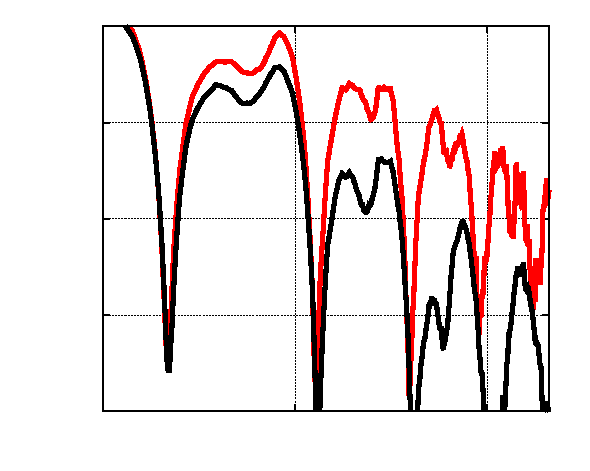
\includegraphics{PSPlainContinuousSAXSIsopoint}}%
    \gplfronttext
  \end{picture}%
\endgroup
}\label{fig:PSPlainContinuousSAXSIsopoint}}
	\caption{PS-Plain continuous contrast variation: a) SAXS curves of PS-Plain obtained by density gradient contrast variation after solvent background subtraction. b) The relative standard
deviation of each $q$ calculated across all the measured scattering curves, where the minima correspond to the isoscattering points $I_i$. The background subtraction shifts the position of $I_i$, especially for high $q$-values.}
\end{figure}

From the 40 experimental scattering curves shown in figure \ref{fig:PSPlainContinuousSAXS}, a model-free size determination can be performed by locating the isoscattering points $I_i$. This is achieved by calculating the relative standard deviation, as shown in figure \ref{fig:PSPlainContinuousSAXSIsopoint}, where the minima correspond to the fulfillment of the isoscattering condition expressed by equation \ref{eq:isoscattering}.

The particle sizes obtained from the first 4 isoscattering points ($I_1$ to $I_4$) range between 142.4 and 144.4 nm, showing a good agreement for higher $q$-values as well. The precision of the isoscattering point positioning decreases for increasing $q$ as demonstrated by Kawaguchi\citep{kawaguchi_isoscattering_1992} and it is exemplified by the broadening of the minima for higher $q$. As observed in figure \ref{fig:PSPlainContinuousSAXSIsopoint}, the effect of the solvent background is relevant principally at high $q$-values as well.

The data can also be analyzed by using the \emph{shape factor} described in section \ref{sec:basic_functions_theory}. The shape factor describes the external shape of the particle independently of its inner structure and is an appropriate approach for the PS-Plain colloid, because it enables the size distribution determination of the particles avoiding any \emph{a priori} consideration about the particle composition.

\begin{figure}
	\begin{center}
		% GNUPLOT: LaTeX picture with Postscript
\begingroup
  \makeatletter
  \providecommand\color[2][]{%
    \GenericError{(gnuplot) \space\space\space\@spaces}{%
      Package color not loaded in conjunction with
      terminal option `colourtext'%
    }{See the gnuplot documentation for explanation.%
    }{Either use 'blacktext' in gnuplot or load the package
      color.sty in LaTeX.}%
    \renewcommand\color[2][]{}%
  }%
  \providecommand\includegraphics[2][]{%
    \GenericError{(gnuplot) \space\space\space\@spaces}{%
      Package graphicx or graphics not loaded%
    }{See the gnuplot documentation for explanation.%
    }{The gnuplot epslatex terminal needs graphicx.sty or graphics.sty.}%
    \renewcommand\includegraphics[2][]{}%
  }%
  \providecommand\rotatebox[2]{#2}%
  \@ifundefined{ifGPcolor}{%
    \newif\ifGPcolor
    \GPcolortrue
  }{}%
  \@ifundefined{ifGPblacktext}{%
    \newif\ifGPblacktext
    \GPblacktextfalse
  }{}%
  % define a \g@addto@macro without @ in the name:
  \let\gplgaddtomacro\g@addto@macro
  % define empty templates for all commands taking text:
  \gdef\gplbacktext{}%
  \gdef\gplfronttext{}%
  \makeatother
  \ifGPblacktext
    % no textcolor at all
    \def\colorrgb#1{}%
    \def\colorgray#1{}%
  \else
    % gray or color?
    \ifGPcolor
      \def\colorrgb#1{\color[rgb]{#1}}%
      \def\colorgray#1{\color[gray]{#1}}%
      \expandafter\def\csname LTw\endcsname{\color{white}}%
      \expandafter\def\csname LTb\endcsname{\color{black}}%
      \expandafter\def\csname LTa\endcsname{\color{black}}%
      \expandafter\def\csname LT0\endcsname{\color[rgb]{1,0,0}}%
      \expandafter\def\csname LT1\endcsname{\color[rgb]{0,1,0}}%
      \expandafter\def\csname LT2\endcsname{\color[rgb]{0,0,1}}%
      \expandafter\def\csname LT3\endcsname{\color[rgb]{1,0,1}}%
      \expandafter\def\csname LT4\endcsname{\color[rgb]{0,1,1}}%
      \expandafter\def\csname LT5\endcsname{\color[rgb]{1,1,0}}%
      \expandafter\def\csname LT6\endcsname{\color[rgb]{0,0,0}}%
      \expandafter\def\csname LT7\endcsname{\color[rgb]{1,0.3,0}}%
      \expandafter\def\csname LT8\endcsname{\color[rgb]{0.5,0.5,0.5}}%
    \else
      % gray
      \def\colorrgb#1{\color{black}}%
      \def\colorgray#1{\color[gray]{#1}}%
      \expandafter\def\csname LTw\endcsname{\color{white}}%
      \expandafter\def\csname LTb\endcsname{\color{black}}%
      \expandafter\def\csname LTa\endcsname{\color{black}}%
      \expandafter\def\csname LT0\endcsname{\color{black}}%
      \expandafter\def\csname LT1\endcsname{\color{black}}%
      \expandafter\def\csname LT2\endcsname{\color{black}}%
      \expandafter\def\csname LT3\endcsname{\color{black}}%
      \expandafter\def\csname LT4\endcsname{\color{black}}%
      \expandafter\def\csname LT5\endcsname{\color{black}}%
      \expandafter\def\csname LT6\endcsname{\color{black}}%
      \expandafter\def\csname LT7\endcsname{\color{black}}%
      \expandafter\def\csname LT8\endcsname{\color{black}}%
    \fi
  \fi
    \setlength{\unitlength}{0.0500bp}%
    \ifx\gptboxheight\undefined%
      \newlength{\gptboxheight}%
      \newlength{\gptboxwidth}%
      \newsavebox{\gptboxtext}%
    \fi%
    \setlength{\fboxrule}{0.5pt}%
    \setlength{\fboxsep}{1pt}%
\begin{picture}(5668.00,4534.00)%
    \gplgaddtomacro\gplbacktext{%
      \csname LTb\endcsname%
      \put(990,704){\makebox(0,0)[r]{\strut{}$1$}}%
      \csname LTb\endcsname%
      \put(990,1377){\makebox(0,0)[r]{\strut{}$10$}}%
      \csname LTb\endcsname%
      \put(990,2049){\makebox(0,0)[r]{\strut{}$100$}}%
      \csname LTb\endcsname%
      \put(990,2722){\makebox(0,0)[r]{\strut{}$1000$}}%
      \csname LTb\endcsname%
      \put(990,3394){\makebox(0,0)[r]{\strut{}$10000$}}%
      \csname LTb\endcsname%
      \put(990,4067){\makebox(0,0)[r]{\strut{}$100000$}}%
      \csname LTb\endcsname%
      \put(1395,484){\makebox(0,0){\strut{}$0.03$}}%
      \csname LTb\endcsname%
      \put(2159,484){\makebox(0,0){\strut{}$0.05$}}%
      \csname LTb\endcsname%
      \put(3197,484){\makebox(0,0){\strut{}$0.1$}}%
      \csname LTb\endcsname%
      \put(4234,484){\makebox(0,0){\strut{}$0.2$}}%
      \csname LTb\endcsname%
      \put(4841,484){\makebox(0,0){\strut{}$0.3$}}%
    }%
    \gplgaddtomacro\gplfronttext{%
      \csname LTb\endcsname%
      \put(220,2486){\rotatebox{-270}{\makebox(0,0){\strut{}Scattering Intensity / a.u.}}}%
      \put(3196,154){\makebox(0,0){\strut{}$q$ / nm$^{-1}$}}%
      \csname LTb\endcsname%
      \put(4548,4041){\makebox(0,0)[r]{\strut{}\smaller Shape scattering function}}%
      \csname LTb\endcsname%
      \put(4548,3711){\makebox(0,0)[r]{\strut{}\smaller Spherical model}}%
    }%
    \gplbacktext
    \put(0,0){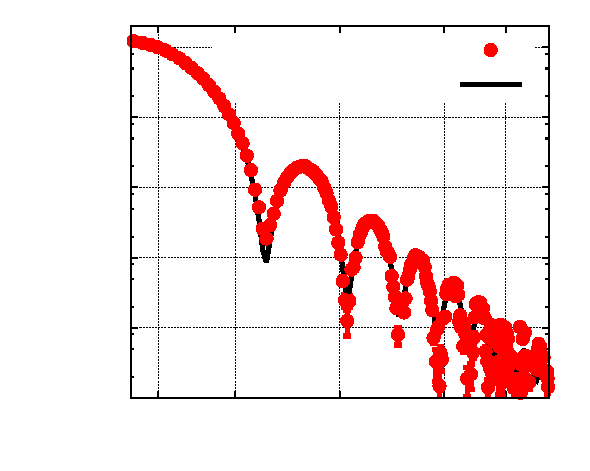
\includegraphics{PSPlainResonantTerm}}%
    \gplfronttext
  \end{picture}%
\endgroup

	\end{center}
	\caption{Experimental shape factor of the PS-Plain colloid calculated from 40 scattering curves and the spherical form factor fitted to the data.}
	\label{fig:PSPlainResonantTerm}
\end{figure}

The shape factor calculated from the measured scattering curves is depicted in figure \ref{fig:PSPlainResonantTerm} together with the spherical model fitted to the data, which employs a simple form factor that ignores the internal structure (eq. \ref{eq:ff_sphere}) and a gaussian size distribution expressed by equation \ref{eq:gauss_distribution}. From this fit, a mean particle size of $(146.8\pm1.3)$ nm was determined. The associated uncertainty calculated with this approach is 3.5 times smaller than the one obtained with the single-contrast SAXS experiment. By fitting the ellipsoid model given by expression \ref{eq:ff_ellipsoid} to the shape factor, a sphericity of $98\;\%$ was obtained.

\subsection{Inter-laboratory comparison of the mean particle diameter}
The improvement in the size accuracy with the shape factor approach is summarized in figure \ref{fig:PSPlainSizeComparison}, where the size of the PS-Plain particles determined by different techniques in an inter-laboratory study is also presented\citep{nicolet_inter-laboratory_2016}.

\begin{figure}
	\centering
		% GNUPLOT: LaTeX picture with Postscript
\begingroup
  \makeatletter
  \providecommand\color[2][]{%
    \GenericError{(gnuplot) \space\space\space\@spaces}{%
      Package color not loaded in conjunction with
      terminal option `colourtext'%
    }{See the gnuplot documentation for explanation.%
    }{Either use 'blacktext' in gnuplot or load the package
      color.sty in LaTeX.}%
    \renewcommand\color[2][]{}%
  }%
  \providecommand\includegraphics[2][]{%
    \GenericError{(gnuplot) \space\space\space\@spaces}{%
      Package graphicx or graphics not loaded%
    }{See the gnuplot documentation for explanation.%
    }{The gnuplot epslatex terminal needs graphicx.sty or graphics.sty.}%
    \renewcommand\includegraphics[2][]{}%
  }%
  \providecommand\rotatebox[2]{#2}%
  \@ifundefined{ifGPcolor}{%
    \newif\ifGPcolor
    \GPcolortrue
  }{}%
  \@ifundefined{ifGPblacktext}{%
    \newif\ifGPblacktext
    \GPblacktextfalse
  }{}%
  % define a \g@addto@macro without @ in the name:
  \let\gplgaddtomacro\g@addto@macro
  % define empty templates for all commands taking text:
  \gdef\gplbacktext{}%
  \gdef\gplfronttext{}%
  \makeatother
  \ifGPblacktext
    % no textcolor at all
    \def\colorrgb#1{}%
    \def\colorgray#1{}%
  \else
    % gray or color?
    \ifGPcolor
      \def\colorrgb#1{\color[rgb]{#1}}%
      \def\colorgray#1{\color[gray]{#1}}%
      \expandafter\def\csname LTw\endcsname{\color{white}}%
      \expandafter\def\csname LTb\endcsname{\color{black}}%
      \expandafter\def\csname LTa\endcsname{\color{black}}%
      \expandafter\def\csname LT0\endcsname{\color[rgb]{1,0,0}}%
      \expandafter\def\csname LT1\endcsname{\color[rgb]{0,1,0}}%
      \expandafter\def\csname LT2\endcsname{\color[rgb]{0,0,1}}%
      \expandafter\def\csname LT3\endcsname{\color[rgb]{1,0,1}}%
      \expandafter\def\csname LT4\endcsname{\color[rgb]{0,1,1}}%
      \expandafter\def\csname LT5\endcsname{\color[rgb]{1,1,0}}%
      \expandafter\def\csname LT6\endcsname{\color[rgb]{0,0,0}}%
      \expandafter\def\csname LT7\endcsname{\color[rgb]{1,0.3,0}}%
      \expandafter\def\csname LT8\endcsname{\color[rgb]{0.5,0.5,0.5}}%
    \else
      % gray
      \def\colorrgb#1{\color{black}}%
      \def\colorgray#1{\color[gray]{#1}}%
      \expandafter\def\csname LTw\endcsname{\color{white}}%
      \expandafter\def\csname LTb\endcsname{\color{black}}%
      \expandafter\def\csname LTa\endcsname{\color{black}}%
      \expandafter\def\csname LT0\endcsname{\color{black}}%
      \expandafter\def\csname LT1\endcsname{\color{black}}%
      \expandafter\def\csname LT2\endcsname{\color{black}}%
      \expandafter\def\csname LT3\endcsname{\color{black}}%
      \expandafter\def\csname LT4\endcsname{\color{black}}%
      \expandafter\def\csname LT5\endcsname{\color{black}}%
      \expandafter\def\csname LT6\endcsname{\color{black}}%
      \expandafter\def\csname LT7\endcsname{\color{black}}%
      \expandafter\def\csname LT8\endcsname{\color{black}}%
    \fi
  \fi
    \setlength{\unitlength}{0.0500bp}%
    \ifx\gptboxheight\undefined%
      \newlength{\gptboxheight}%
      \newlength{\gptboxwidth}%
      \newsavebox{\gptboxtext}%
    \fi%
    \setlength{\fboxrule}{0.5pt}%
    \setlength{\fboxsep}{1pt}%
\begin{picture}(5668.00,4534.00)%
    \gplgaddtomacro\gplbacktext{%
      \csname LTb\endcsname%
      \put(682,1869){\makebox(0,0)[r]{\strut{}$130$}}%
      \csname LTb\endcsname%
      \put(682,2297){\makebox(0,0)[r]{\strut{}$135$}}%
      \csname LTb\endcsname%
      \put(682,2726){\makebox(0,0)[r]{\strut{}$140$}}%
      \csname LTb\endcsname%
      \put(682,3155){\makebox(0,0)[r]{\strut{}$145$}}%
      \csname LTb\endcsname%
      \put(682,3583){\makebox(0,0)[r]{\strut{}$150$}}%
      \csname LTb\endcsname%
      \put(682,4012){\makebox(0,0)[r]{\strut{}$155$}}%
      \csname LTb\endcsname%
      \put(1054,1394){\rotatebox{-45}{\makebox(0,0)[l]{\strut{}AFM (SMD)}}}%
      \csname LTb\endcsname%
      \put(1533,1394){\rotatebox{-45}{\makebox(0,0)[l]{\strut{}AFM (METAS)}}}%
      \csname LTb\endcsname%
      \put(2012,1394){\rotatebox{-45}{\makebox(0,0)[l]{\strut{}AFM (VSL)}}}%
      \csname LTb\endcsname%
      \put(2491,1394){\rotatebox{-45}{\makebox(0,0)[l]{\strut{}TSEM}}}%
      \csname LTb\endcsname%
      \put(2971,1394){\rotatebox{-45}{\makebox(0,0)[l]{\strut{}DCS}}}%
      \csname LTb\endcsname%
      \put(3450,1394){\rotatebox{-45}{\makebox(0,0)[l]{\strut{}Core-shell}}}%
      \csname LTb\endcsname%
      \put(3929,1394){\rotatebox{-45}{\makebox(0,0)[l]{\strut{}Shape function}}}%
      \csname LTb\endcsname%
      \put(4313,1394){\rotatebox{-45}{\makebox(0,0)[l]{\strut{}$I_1$}}}%
      \csname LTb\endcsname%
      \put(4552,1394){\rotatebox{-45}{\makebox(0,0)[l]{\strut{}$I_2$}}}%
      \csname LTb\endcsname%
      \put(4792,1394){\rotatebox{-45}{\makebox(0,0)[l]{\strut{}$I_3$}}}%
      \csname LTb\endcsname%
      \put(5031,1394){\rotatebox{-45}{\makebox(0,0)[l]{\strut{}$I_4$}}}%
    }%
    \gplgaddtomacro\gplfronttext{%
      \csname LTb\endcsname%
      \put(176,2897){\rotatebox{-270}{\makebox(0,0){\strut{}Diameter / nm}}}%
    }%
    \gplbacktext
    \put(0,0){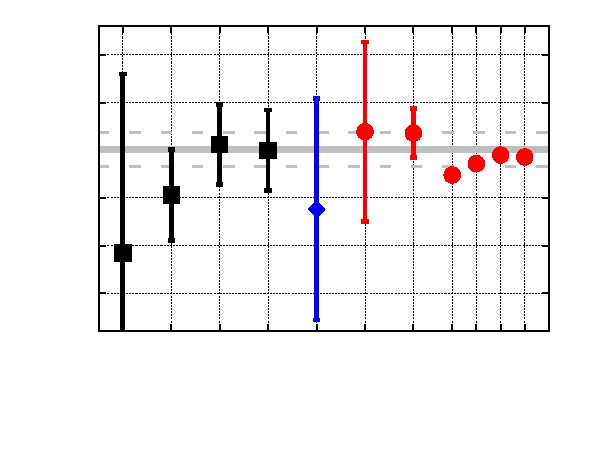
\includegraphics{PSPlainSizeComparison}}%
    \gplfronttext
  \end{picture}%
\endgroup

	\caption{Comparison of the PS-Plain average size obtained with different techniques, where the errorbars correspond to the expanded uncertainty ($k=2$). The circles correspond to results obtained with SAXS and the diamonds to combined DCS measurements. The gray line defines the weighted mean of all the independent results. The microscopy values are obtained from Belgian Service Métrologie-Metrologische Dienst (SMD), Swiss Federal Institute of Metrology (METAS) and Dutch Metrology Institute (VSL).}
	\label{fig:PSPlainSizeComparison}
\end{figure}

The figure compares the PS-Plain size measured by the ensemble techniques SAXS and DCS and the imaging methods AFM and TSEM and presents the weighted mean value of all the independent results as a grey line, which corresponds to a diameter of 145.1 nm with an associated expanded uncertainty ($k=2$) of 1.8 nm. The SAXS results tend to larger values when modelling the scattering form factor, whilst the size obtained from the isoscattering points positions $I_i$ present values slightly smaller than the calculated mean value. However, the maximum deviation from the weighted mean is less than 2 $\%$.

The DCS result is obtained by a combined analysis of two complementary centrifuge configurations as detailed in section \ref{sec:DCS_experimental}, where figure \ref{fig:DCSCombinedStokes} depicts the dependency of the measured particle size on the density values for the two setups. The two setups measure the same size and density at the crossing point of the data, which occurs for a diameter of ($138.8\pm5.8$) nm and a density of ($1.052\pm0.010$) g cm$^{-3}$. The measured size fits within its uncertainty in the confidence interval of one standard deviation of the inter-laboratory comparison.

\begin{figure}
	\begin{center}
		% GNUPLOT: LaTeX picture with Postscript
\begingroup
  \makeatletter
  \providecommand\color[2][]{%
    \GenericError{(gnuplot) \space\space\space\@spaces}{%
      Package color not loaded in conjunction with
      terminal option `colourtext'%
    }{See the gnuplot documentation for explanation.%
    }{Either use 'blacktext' in gnuplot or load the package
      color.sty in LaTeX.}%
    \renewcommand\color[2][]{}%
  }%
  \providecommand\includegraphics[2][]{%
    \GenericError{(gnuplot) \space\space\space\@spaces}{%
      Package graphicx or graphics not loaded%
    }{See the gnuplot documentation for explanation.%
    }{The gnuplot epslatex terminal needs graphicx.sty or graphics.sty.}%
    \renewcommand\includegraphics[2][]{}%
  }%
  \providecommand\rotatebox[2]{#2}%
  \@ifundefined{ifGPcolor}{%
    \newif\ifGPcolor
    \GPcolortrue
  }{}%
  \@ifundefined{ifGPblacktext}{%
    \newif\ifGPblacktext
    \GPblacktextfalse
  }{}%
  % define a \g@addto@macro without @ in the name:
  \let\gplgaddtomacro\g@addto@macro
  % define empty templates for all commands taking text:
  \gdef\gplbacktext{}%
  \gdef\gplfronttext{}%
  \makeatother
  \ifGPblacktext
    % no textcolor at all
    \def\colorrgb#1{}%
    \def\colorgray#1{}%
  \else
    % gray or color?
    \ifGPcolor
      \def\colorrgb#1{\color[rgb]{#1}}%
      \def\colorgray#1{\color[gray]{#1}}%
      \expandafter\def\csname LTw\endcsname{\color{white}}%
      \expandafter\def\csname LTb\endcsname{\color{black}}%
      \expandafter\def\csname LTa\endcsname{\color{black}}%
      \expandafter\def\csname LT0\endcsname{\color[rgb]{1,0,0}}%
      \expandafter\def\csname LT1\endcsname{\color[rgb]{0,1,0}}%
      \expandafter\def\csname LT2\endcsname{\color[rgb]{0,0,1}}%
      \expandafter\def\csname LT3\endcsname{\color[rgb]{1,0,1}}%
      \expandafter\def\csname LT4\endcsname{\color[rgb]{0,1,1}}%
      \expandafter\def\csname LT5\endcsname{\color[rgb]{1,1,0}}%
      \expandafter\def\csname LT6\endcsname{\color[rgb]{0,0,0}}%
      \expandafter\def\csname LT7\endcsname{\color[rgb]{1,0.3,0}}%
      \expandafter\def\csname LT8\endcsname{\color[rgb]{0.5,0.5,0.5}}%
    \else
      % gray
      \def\colorrgb#1{\color{black}}%
      \def\colorgray#1{\color[gray]{#1}}%
      \expandafter\def\csname LTw\endcsname{\color{white}}%
      \expandafter\def\csname LTb\endcsname{\color{black}}%
      \expandafter\def\csname LTa\endcsname{\color{black}}%
      \expandafter\def\csname LT0\endcsname{\color{black}}%
      \expandafter\def\csname LT1\endcsname{\color{black}}%
      \expandafter\def\csname LT2\endcsname{\color{black}}%
      \expandafter\def\csname LT3\endcsname{\color{black}}%
      \expandafter\def\csname LT4\endcsname{\color{black}}%
      \expandafter\def\csname LT5\endcsname{\color{black}}%
      \expandafter\def\csname LT6\endcsname{\color{black}}%
      \expandafter\def\csname LT7\endcsname{\color{black}}%
      \expandafter\def\csname LT8\endcsname{\color{black}}%
    \fi
  \fi
  \setlength{\unitlength}{0.0500bp}%
  \begin{picture}(5668.00,4534.00)%
    \gplgaddtomacro\gplbacktext{%
      \csname LTb\endcsname%
      \put(880,1232){\makebox(0,0)[r]{\strut{} 100}}%
      \csname LTb\endcsname%
      \put(880,1892){\makebox(0,0)[r]{\strut{} 150}}%
      \csname LTb\endcsname%
      \put(880,2553){\makebox(0,0)[r]{\strut{} 200}}%
      \csname LTb\endcsname%
      \put(880,3213){\makebox(0,0)[r]{\strut{} 250}}%
      \csname LTb\endcsname%
      \put(880,3873){\makebox(0,0)[r]{\strut{} 300}}%
      \csname LTb\endcsname%
      \put(1367,484){\makebox(0,0){\strut{} 1.02}}%
      \csname LTb\endcsname%
      \put(2077,484){\makebox(0,0){\strut{} 1.04}}%
      \csname LTb\endcsname%
      \put(2787,484){\makebox(0,0){\strut{} 1.06}}%
      \csname LTb\endcsname%
      \put(3496,484){\makebox(0,0){\strut{} 1.08}}%
      \csname LTb\endcsname%
      \put(4206,484){\makebox(0,0){\strut{} 1.1}}%
      \csname LTb\endcsname%
      \put(4916,484){\makebox(0,0){\strut{} 1.12}}%
      \put(176,2486){\rotatebox{-270}{\makebox(0,0){\strut{}PS-Plain diameter / nm}}}%
      \put(3141,154){\makebox(0,0){\strut{}PS-Plain density / g cm$^{-3}$}}%
    }%
    \gplgaddtomacro\gplfronttext{%
      \csname LTb\endcsname%
      \put(3793,4038){\makebox(0,0)[r]{\strut{}\smaller Standard disc}}%
      \csname LTb\endcsname%
      \put(3793,3708){\makebox(0,0)[r]{\strut{}\smaller Low density disc}}%
    }%
    \gplbacktext
    \put(0,0){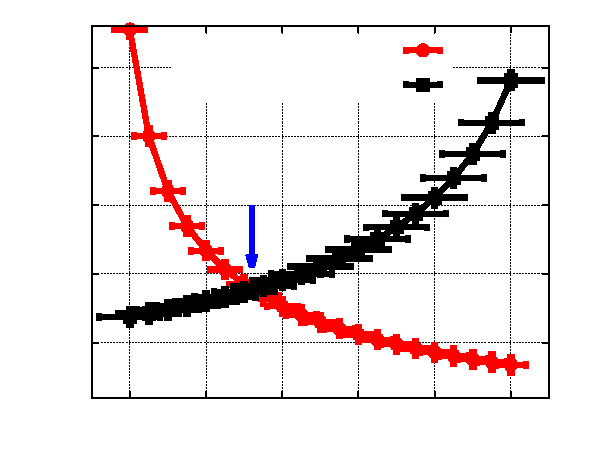
\includegraphics{DCSCombinedStokes}}%
    \gplfronttext
  \end{picture}%
\endgroup

	\end{center}
	\caption{Dependence of the intensity-based modal Stokes' diameter on the particle density for PS-Plain particles analyzed in H$_2$O-sucrose (black) and D$_2$O-sucrose (red) gradients. The arrow indicates the crossing point of the data, where the two setups measure the same size and density of the colloid. This occurs for a diameter of ($138.8\pm5.8$) nm and a density of ($1.052\pm0.010$) g cm$^{-3}$}
	\label{fig:DCSCombinedStokes}
\end{figure}
 
All the techniques are in very good agreement, even considering that they are based on different physical principles. The improvement in accuracy for the size determination with SAXS by using the shape factor approach is further sustained by this comparison. 

This improvement was confirmed by employing the same approach with the PS-COOH colloids. The size obtained from the core-shell model fit in chapter \ref{chap:density_gradient_SAXS} is ($99.4\pm5.6$) nm, while the value obtained from the shape factor calculation is ($101.4\pm2.4$) nm. Again, the uncertainty associated to the size decreases by $\sim 60\;\%$, whilst it is still in accordance with the size obtained with the isoscattering points positions of 101.0 nm with a standard deviation of 1.1 nm. 

Due to the low polydispersity of the PMMA-COOH particles and their homogenous composition, a spherical form factor fit to the single-contrast scattering curve provides already a very accurate size ($186.5\pm2.3$) nm. In this case, contrast variation experiments in SAXS show no advantadges.

\subsection{Particle size distribution of PS-Plain}

An important attribute of polymeric colloids is their polydispersity, as the suitability for specific applications depends on their spread in size. For example, colloids are known to induce different inflammatory responses depending on their size\citep{kusaka_effect_2014}.

\begin{figure}
	\begin{center}
		% GNUPLOT: LaTeX picture with Postscript
\begingroup
  \makeatletter
  \providecommand\color[2][]{%
    \GenericError{(gnuplot) \space\space\space\@spaces}{%
      Package color not loaded in conjunction with
      terminal option `colourtext'%
    }{See the gnuplot documentation for explanation.%
    }{Either use 'blacktext' in gnuplot or load the package
      color.sty in LaTeX.}%
    \renewcommand\color[2][]{}%
  }%
  \providecommand\includegraphics[2][]{%
    \GenericError{(gnuplot) \space\space\space\@spaces}{%
      Package graphicx or graphics not loaded%
    }{See the gnuplot documentation for explanation.%
    }{The gnuplot epslatex terminal needs graphicx.sty or graphics.sty.}%
    \renewcommand\includegraphics[2][]{}%
  }%
  \providecommand\rotatebox[2]{#2}%
  \@ifundefined{ifGPcolor}{%
    \newif\ifGPcolor
    \GPcolortrue
  }{}%
  \@ifundefined{ifGPblacktext}{%
    \newif\ifGPblacktext
    \GPblacktextfalse
  }{}%
  % define a \g@addto@macro without @ in the name:
  \let\gplgaddtomacro\g@addto@macro
  % define empty templates for all commands taking text:
  \gdef\gplbacktext{}%
  \gdef\gplfronttext{}%
  \makeatother
  \ifGPblacktext
    % no textcolor at all
    \def\colorrgb#1{}%
    \def\colorgray#1{}%
  \else
    % gray or color?
    \ifGPcolor
      \def\colorrgb#1{\color[rgb]{#1}}%
      \def\colorgray#1{\color[gray]{#1}}%
      \expandafter\def\csname LTw\endcsname{\color{white}}%
      \expandafter\def\csname LTb\endcsname{\color{black}}%
      \expandafter\def\csname LTa\endcsname{\color{black}}%
      \expandafter\def\csname LT0\endcsname{\color[rgb]{1,0,0}}%
      \expandafter\def\csname LT1\endcsname{\color[rgb]{0,1,0}}%
      \expandafter\def\csname LT2\endcsname{\color[rgb]{0,0,1}}%
      \expandafter\def\csname LT3\endcsname{\color[rgb]{1,0,1}}%
      \expandafter\def\csname LT4\endcsname{\color[rgb]{0,1,1}}%
      \expandafter\def\csname LT5\endcsname{\color[rgb]{1,1,0}}%
      \expandafter\def\csname LT6\endcsname{\color[rgb]{0,0,0}}%
      \expandafter\def\csname LT7\endcsname{\color[rgb]{1,0.3,0}}%
      \expandafter\def\csname LT8\endcsname{\color[rgb]{0.5,0.5,0.5}}%
    \else
      % gray
      \def\colorrgb#1{\color{black}}%
      \def\colorgray#1{\color[gray]{#1}}%
      \expandafter\def\csname LTw\endcsname{\color{white}}%
      \expandafter\def\csname LTb\endcsname{\color{black}}%
      \expandafter\def\csname LTa\endcsname{\color{black}}%
      \expandafter\def\csname LT0\endcsname{\color{black}}%
      \expandafter\def\csname LT1\endcsname{\color{black}}%
      \expandafter\def\csname LT2\endcsname{\color{black}}%
      \expandafter\def\csname LT3\endcsname{\color{black}}%
      \expandafter\def\csname LT4\endcsname{\color{black}}%
      \expandafter\def\csname LT5\endcsname{\color{black}}%
      \expandafter\def\csname LT6\endcsname{\color{black}}%
      \expandafter\def\csname LT7\endcsname{\color{black}}%
      \expandafter\def\csname LT8\endcsname{\color{black}}%
    \fi
  \fi
  \setlength{\unitlength}{0.0500bp}%
  \begin{picture}(5668.00,4534.00)%
    \gplgaddtomacro\gplbacktext{%
      \csname LTb\endcsname%
      \put(814,777){\makebox(0,0)[r]{\strut{} 0}}%
      \csname LTb\endcsname%
      \put(814,1359){\makebox(0,0)[r]{\strut{} 0.2}}%
      \csname LTb\endcsname%
      \put(814,1941){\makebox(0,0)[r]{\strut{} 0.4}}%
      \csname LTb\endcsname%
      \put(814,2523){\makebox(0,0)[r]{\strut{} 0.6}}%
      \csname LTb\endcsname%
      \put(814,3105){\makebox(0,0)[r]{\strut{} 0.8}}%
      \csname LTb\endcsname%
      \put(814,3687){\makebox(0,0)[r]{\strut{} 1}}%
      \csname LTb\endcsname%
      \put(814,4269){\makebox(0,0)[r]{\strut{} 1.2}}%
      \csname LTb\endcsname%
      \put(946,484){\makebox(0,0){\strut{} 80}}%
      \csname LTb\endcsname%
      \put(1732,484){\makebox(0,0){\strut{} 100}}%
      \csname LTb\endcsname%
      \put(2519,484){\makebox(0,0){\strut{} 120}}%
      \csname LTb\endcsname%
      \put(3305,484){\makebox(0,0){\strut{} 140}}%
      \csname LTb\endcsname%
      \put(4091,484){\makebox(0,0){\strut{} 160}}%
      \csname LTb\endcsname%
      \put(4878,484){\makebox(0,0){\strut{} 180}}%
      \put(176,2486){\rotatebox{-270}{\makebox(0,0){\strut{}Frequency / a.u.}}}%
      \put(3108,154){\makebox(0,0){\strut{}Size / nm}}%
    }%
    \gplgaddtomacro\gplfronttext{%
      \csname LTb\endcsname%
      \put(2371,4046){\makebox(0,0)[r]{\strut{}TSEM}}%
      \csname LTb\endcsname%
      \put(2371,3716){\makebox(0,0)[r]{\strut{}Shape Factor SAXS}}%
      \csname LTb\endcsname%
      \put(2371,3386){\makebox(0,0)[r]{\strut{}Standard DCS}}%
      \csname LTb\endcsname%
      \put(2371,3056){\makebox(0,0)[r]{\strut{}Low density DCS}}%
    }%
    \gplbacktext
    \put(0,0){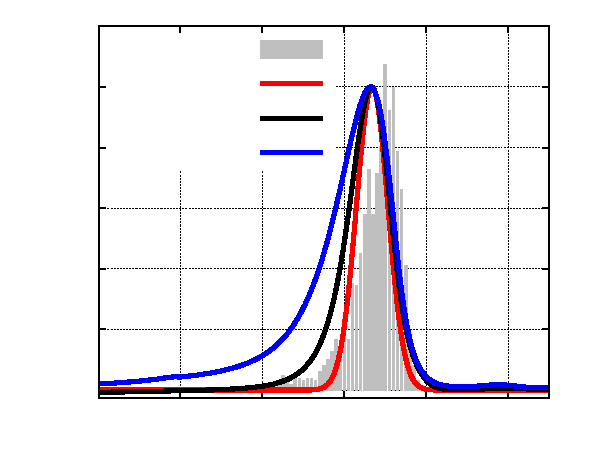
\includegraphics{PSPlainSizeDistribution}}%
    \gplfronttext
  \end{picture}%
\endgroup

	\end{center}
	\caption{Number-weighted size distribution of PS-Plain particles measured by DCS, TSEM \citep{nicolet_inter-laboratory_2016} and SAXS with the scattering shape factor approach.}
	\label{fig:PSPlainSizeDistribution}
\end{figure}

The SAXS results determine a polydispersity degree $p_d$ for the PS-Plain colloids of 6.1 $\%$, which is an indicator of a very monodisperse distribution, as also suggested by the regular minima observed in figure \ref{fig:PSPlainSingleContrastSAXS}. Particle polydispersities measured by DCS are also low as observed in figure \ref{fig:PSPlainSizeDistribution}, ranging from 7.8 $\%$ measured with the standard set up, to 11.3 $\%$ measured with the low density disc setup. The standard setup appears therefore to achieve a higher resolution size distribution. The size distribution measured by TSEM with a $p_d$ of 8.3 $\%$ shows good agreement with the ensemble techniques.

The measurements obtained by AFM provide polydispersity degrees larger than 10 $\%$\citep{nicolet_inter-laboratory_2016} and, therefore, slightly broader size distributions than those calculated by SAXS, TSEM and standard DCS. This can be in part attributed to the low statistics that typically affect imaging methods, along with artefacts associated with the posterior analysis.

For instance, in the TSEM images\citep{nicolet_inter-laboratory_2016}, smaller and larger populations with different contrasts have been observed which could affect the evaluation of the density measured by ensemble techniques in the following section \ref{sec:physical_density}, as the particle average density might vary. Indeed, when a bimodal distribution is used to analyze the SAXS shape factor of PS-Plain particles, a second size population is found at 101 nm in agreement with TSEM, while the main mode maintains a $p_d$ of ca. 5 $\%$.

\section{Considerations about scattering data evaluation}

In the previous section, the mean diameter of polymeric nanoparticles was obtained using two different model-free approaches, i.e. the isoscattering point and the shape factor. The method employed to analyze the scattering curves measured with the continuous contrast variation technique in SAXS affects the size determination and its accuracy, as suggested by the results. Following, a discussion about both approaches is presented based on the scattering data shown in figure \ref{fig:PSPlainContinuousSAXS}.

\subsection{Shape factor formalism}
The shape factor obtained by density gradient contrast variation has been demonstrated as a powerful technique which can provide precise information about the size distribution and shape of the colloid by fitting a simple form factor.

\begin{figure}
	\begin{center}
		% GNUPLOT: LaTeX picture with Postscript
\begingroup
  \makeatletter
  \providecommand\color[2][]{%
    \GenericError{(gnuplot) \space\space\space\@spaces}{%
      Package color not loaded in conjunction with
      terminal option `colourtext'%
    }{See the gnuplot documentation for explanation.%
    }{Either use 'blacktext' in gnuplot or load the package
      color.sty in LaTeX.}%
    \renewcommand\color[2][]{}%
  }%
  \providecommand\includegraphics[2][]{%
    \GenericError{(gnuplot) \space\space\space\@spaces}{%
      Package graphicx or graphics not loaded%
    }{See the gnuplot documentation for explanation.%
    }{The gnuplot epslatex terminal needs graphicx.sty or graphics.sty.}%
    \renewcommand\includegraphics[2][]{}%
  }%
  \providecommand\rotatebox[2]{#2}%
  \@ifundefined{ifGPcolor}{%
    \newif\ifGPcolor
    \GPcolortrue
  }{}%
  \@ifundefined{ifGPblacktext}{%
    \newif\ifGPblacktext
    \GPblacktextfalse
  }{}%
  % define a \g@addto@macro without @ in the name:
  \let\gplgaddtomacro\g@addto@macro
  % define empty templates for all commands taking text:
  \gdef\gplbacktext{}%
  \gdef\gplfronttext{}%
  \makeatother
  \ifGPblacktext
    % no textcolor at all
    \def\colorrgb#1{}%
    \def\colorgray#1{}%
  \else
    % gray or color?
    \ifGPcolor
      \def\colorrgb#1{\color[rgb]{#1}}%
      \def\colorgray#1{\color[gray]{#1}}%
      \expandafter\def\csname LTw\endcsname{\color{white}}%
      \expandafter\def\csname LTb\endcsname{\color{black}}%
      \expandafter\def\csname LTa\endcsname{\color{black}}%
      \expandafter\def\csname LT0\endcsname{\color[rgb]{1,0,0}}%
      \expandafter\def\csname LT1\endcsname{\color[rgb]{0,1,0}}%
      \expandafter\def\csname LT2\endcsname{\color[rgb]{0,0,1}}%
      \expandafter\def\csname LT3\endcsname{\color[rgb]{1,0,1}}%
      \expandafter\def\csname LT4\endcsname{\color[rgb]{0,1,1}}%
      \expandafter\def\csname LT5\endcsname{\color[rgb]{1,1,0}}%
      \expandafter\def\csname LT6\endcsname{\color[rgb]{0,0,0}}%
      \expandafter\def\csname LT7\endcsname{\color[rgb]{1,0.3,0}}%
      \expandafter\def\csname LT8\endcsname{\color[rgb]{0.5,0.5,0.5}}%
    \else
      % gray
      \def\colorrgb#1{\color{black}}%
      \def\colorgray#1{\color[gray]{#1}}%
      \expandafter\def\csname LTw\endcsname{\color{white}}%
      \expandafter\def\csname LTb\endcsname{\color{black}}%
      \expandafter\def\csname LTa\endcsname{\color{black}}%
      \expandafter\def\csname LT0\endcsname{\color{black}}%
      \expandafter\def\csname LT1\endcsname{\color{black}}%
      \expandafter\def\csname LT2\endcsname{\color{black}}%
      \expandafter\def\csname LT3\endcsname{\color{black}}%
      \expandafter\def\csname LT4\endcsname{\color{black}}%
      \expandafter\def\csname LT5\endcsname{\color{black}}%
      \expandafter\def\csname LT6\endcsname{\color{black}}%
      \expandafter\def\csname LT7\endcsname{\color{black}}%
      \expandafter\def\csname LT8\endcsname{\color{black}}%
    \fi
  \fi
  \setlength{\unitlength}{0.0500bp}%
  \begin{picture}(5668.00,4534.00)%
    \gplgaddtomacro\gplbacktext{%
      \csname LTb\endcsname%
      \put(748,866){\makebox(0,0)[r]{\strut{} 140}}%
      \csname LTb\endcsname%
      \put(748,1514){\makebox(0,0)[r]{\strut{} 142}}%
      \csname LTb\endcsname%
      \put(748,2162){\makebox(0,0)[r]{\strut{} 144}}%
      \csname LTb\endcsname%
      \put(748,2811){\makebox(0,0)[r]{\strut{} 146}}%
      \csname LTb\endcsname%
      \put(748,3459){\makebox(0,0)[r]{\strut{} 148}}%
      \csname LTb\endcsname%
      \put(748,4107){\makebox(0,0)[r]{\strut{} 150}}%
      \csname LTb\endcsname%
      \put(880,484){\makebox(0,0){\strut{} 0}}%
      \csname LTb\endcsname%
      \put(1507,484){\makebox(0,0){\strut{} 5}}%
      \csname LTb\endcsname%
      \put(2135,484){\makebox(0,0){\strut{} 10}}%
      \csname LTb\endcsname%
      \put(2762,484){\makebox(0,0){\strut{} 15}}%
      \csname LTb\endcsname%
      \put(3389,484){\makebox(0,0){\strut{} 20}}%
      \csname LTb\endcsname%
      \put(4016,484){\makebox(0,0){\strut{} 25}}%
      \csname LTb\endcsname%
      \put(4644,484){\makebox(0,0){\strut{} 30}}%
      \csname LTb\endcsname%
      \put(5271,484){\makebox(0,0){\strut{} 35}}%
      \put(176,2486){\rotatebox{-270}{\makebox(0,0){\strut{}Diameter / nm}}}%
      \put(3075,154){\makebox(0,0){\strut{}Number of scattering curves}}%
    }%
    \gplgaddtomacro\gplfronttext{%
    }%
    \gplbacktext
    \put(0,0){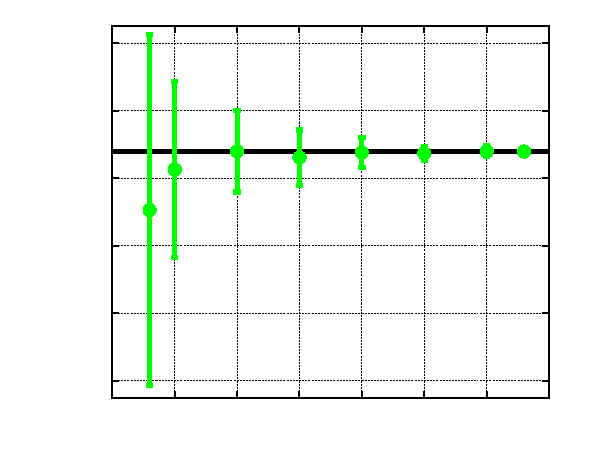
\includegraphics{ResonantTermSimulationNumber}}%
    \gplfronttext
  \end{picture}%
\endgroup

	\end{center}
\caption{Size of PS-Plain as a function of the number of scattering curves used in the shape factor calculation. The horizontal lines lies at 146.8 nm.}
\label{fig:ResonantTermSimulationNumber}
\end{figure}

However, an accurate determination of the suspending medium density for each scattering curve is required, due to the increased uncertainties\citep{lefebvre_propagation_2000} that can arise from the resolution of the system of linear equations described in section \ref{sec:basic_functions_theory}.

Besides, a minimum of 3 scattering curves measured at different contrasts is necessary to obtain the resonant term, although an increasing number improves the determination of the size distribution. This issue has been adressed with the data measured by the density gradient contrast variation of the PS-Plain colloid. 

From the 40 experimental curves, only a limited number $N$ was randomly selected to compute the shape factor, while this process was repeated 100 times. The mean size obtained from this data set and its standard deviation are plotted in figure \ref{fig:ResonantTermSimulationNumber} as a function of $N$.

The effect of increasing the number of measured contrasts evidences that the result tends asymptotically to the value of 146.8 nm discussed in section \ref{sec:size_validation} and the standard deviation of the 100 iterations decreases for large $N$, e.g. the associated uncertainty is reduced. This outcome emphasizes further the advantages of the continuous contrast variation technique due to the large number of scattering curves at different contrasts which can be easily measured.

In summary, it has been demonstrated that the possibility to determine the particle size distribution by the scattering shape factor is a clear improvement to single-contrast SAXS techniques reducing relevantly the uncertainty, although an accurate determination of the contrast and a relatively high number of scattering curves are required. 

\subsection{Isoscattering point approach}

The theory defines $q^{\star}$ as a morphological parameter independent of the suspending medium density, which is a enormous practical advantage as it can be located without the proper calibration of the contrast. In cases where the composition of the buffer is unknown or the density of the solvent cannot be properly calibrated, the isoscattering point position might still be quantifiable by calculating the relative standard deviation of all the measured scattering curves. 

In order to obtain reliable results, a proper subtraction of the solvent scattering must be performed. It is clear in figure \ref{fig:PSPlainContinuousSAXSIsopoint} that the correction of the solvent contribution to the scattering intensity plays an important role in the determination of the $q^{\star}$ values as the curve shifts to smaller $q$-values when subtracting the solvent background. Although this effect is larger at high $q$-values, the solvent background influences the position of all the isoscattering points as summarized in table \ref{tab:isoscattering_points}. 

\begin{table}
	\centering
	\begin{tabular}{l||cc|cc|c}
		 & \multicolumn{2}{c}{Raw data} & \multicolumn{2}{c}{Corrected data} & Deviation\\
		 \hline
		 & \( q^{\star} \) (nm\(^{-1}\))    &  Size (nm) & \( q^{\star}\) (nm\(^{-1}\))    &  Size (nm) & $\%$ \\
		\hline
		 \(q^{\star}_1\) &  0.0633 & 142.0 &  0.0631 & 142.4 & 0.3 \\
		 \(q^{\star}_2\) &  0.1088 & 142.0 &  0.1076 & 143.6 & 1.1   \\
		 \(q^{\star}_3\) &  0.1537 & 141.9 &  0.1510 & 144.4 & 1.7    \\
		 \(q^{\star}_4\) &  0.206  & 136.6 &  0.195  & 144.3 & 5.3     \\
		\end{tabular}
	\caption{Isoscattering points position and the corresponding particle size for the scattering curves before and after background correction. The size deviation between both values is also shown, with larger deviation for higher $q$-values.}
	\label{tab:isoscattering_points}
\end{table}

It has been discussed before in this work that the polydispersity of the latex and its deviation from the spherical shape influence the position and diffuseness of $q^{\star}$, principally at high $q$-values. This can disturb the size determination for polymeric particles with broad size distributions and limit the applicability of this technique. 

\textcolor{blue}{In figure \ref{fig:IsopointSimulationPolydispersity}, the diameter obtained from the first isoscattering point position is simulated for three core-shell particle with different core-to-size ratios. The deviation of the measured size from the nominal size becomes larger for increasing particle polydispersities, reaching size deviations up to 8 $\%$ at $p_d = 30\;\%$. Moreover, the size deviation behaves differently depending on the internal structure of the particle, tending to larger deviations for thicker shells and positive deviations for thinner ones.}

\begin{figure}%[htbp]
	\centering
		\subfloat[Polydispersity effects]{\resizebox{0.44\linewidth}{!}{% GNUPLOT: LaTeX picture with Postscript
\begingroup
  \makeatletter
  \providecommand\color[2][]{%
    \GenericError{(gnuplot) \space\space\space\@spaces}{%
      Package color not loaded in conjunction with
      terminal option `colourtext'%
    }{See the gnuplot documentation for explanation.%
    }{Either use 'blacktext' in gnuplot or load the package
      color.sty in LaTeX.}%
    \renewcommand\color[2][]{}%
  }%
  \providecommand\includegraphics[2][]{%
    \GenericError{(gnuplot) \space\space\space\@spaces}{%
      Package graphicx or graphics not loaded%
    }{See the gnuplot documentation for explanation.%
    }{The gnuplot epslatex terminal needs graphicx.sty or graphics.sty.}%
    \renewcommand\includegraphics[2][]{}%
  }%
  \providecommand\rotatebox[2]{#2}%
  \@ifundefined{ifGPcolor}{%
    \newif\ifGPcolor
    \GPcolortrue
  }{}%
  \@ifundefined{ifGPblacktext}{%
    \newif\ifGPblacktext
    \GPblacktextfalse
  }{}%
  % define a \g@addto@macro without @ in the name:
  \let\gplgaddtomacro\g@addto@macro
  % define empty templates for all commands taking text:
  \gdef\gplbacktext{}%
  \gdef\gplfronttext{}%
  \makeatother
  \ifGPblacktext
    % no textcolor at all
    \def\colorrgb#1{}%
    \def\colorgray#1{}%
  \else
    % gray or color?
    \ifGPcolor
      \def\colorrgb#1{\color[rgb]{#1}}%
      \def\colorgray#1{\color[gray]{#1}}%
      \expandafter\def\csname LTw\endcsname{\color{white}}%
      \expandafter\def\csname LTb\endcsname{\color{black}}%
      \expandafter\def\csname LTa\endcsname{\color{black}}%
      \expandafter\def\csname LT0\endcsname{\color[rgb]{1,0,0}}%
      \expandafter\def\csname LT1\endcsname{\color[rgb]{0,1,0}}%
      \expandafter\def\csname LT2\endcsname{\color[rgb]{0,0,1}}%
      \expandafter\def\csname LT3\endcsname{\color[rgb]{1,0,1}}%
      \expandafter\def\csname LT4\endcsname{\color[rgb]{0,1,1}}%
      \expandafter\def\csname LT5\endcsname{\color[rgb]{1,1,0}}%
      \expandafter\def\csname LT6\endcsname{\color[rgb]{0,0,0}}%
      \expandafter\def\csname LT7\endcsname{\color[rgb]{1,0.3,0}}%
      \expandafter\def\csname LT8\endcsname{\color[rgb]{0.5,0.5,0.5}}%
    \else
      % gray
      \def\colorrgb#1{\color{black}}%
      \def\colorgray#1{\color[gray]{#1}}%
      \expandafter\def\csname LTw\endcsname{\color{white}}%
      \expandafter\def\csname LTb\endcsname{\color{black}}%
      \expandafter\def\csname LTa\endcsname{\color{black}}%
      \expandafter\def\csname LT0\endcsname{\color{black}}%
      \expandafter\def\csname LT1\endcsname{\color{black}}%
      \expandafter\def\csname LT2\endcsname{\color{black}}%
      \expandafter\def\csname LT3\endcsname{\color{black}}%
      \expandafter\def\csname LT4\endcsname{\color{black}}%
      \expandafter\def\csname LT5\endcsname{\color{black}}%
      \expandafter\def\csname LT6\endcsname{\color{black}}%
      \expandafter\def\csname LT7\endcsname{\color{black}}%
      \expandafter\def\csname LT8\endcsname{\color{black}}%
    \fi
  \fi
  \setlength{\unitlength}{0.0500bp}%
  \begin{picture}(5668.00,4534.00)%
    \gplgaddtomacro\gplbacktext{%
      \csname LTb\endcsname%
      \put(682,704){\makebox(0,0)[r]{\strut{}-8}}%
      \csname LTb\endcsname%
      \put(682,1028){\makebox(0,0)[r]{\strut{}-7}}%
      \csname LTb\endcsname%
      \put(682,1352){\makebox(0,0)[r]{\strut{}-6}}%
      \csname LTb\endcsname%
      \put(682,1676){\makebox(0,0)[r]{\strut{}-5}}%
      \csname LTb\endcsname%
      \put(682,2000){\makebox(0,0)[r]{\strut{}-4}}%
      \csname LTb\endcsname%
      \put(682,2324){\makebox(0,0)[r]{\strut{}-3}}%
      \csname LTb\endcsname%
      \put(682,2649){\makebox(0,0)[r]{\strut{}-2}}%
      \csname LTb\endcsname%
      \put(682,2973){\makebox(0,0)[r]{\strut{}-1}}%
      \csname LTb\endcsname%
      \put(682,3297){\makebox(0,0)[r]{\strut{} 0}}%
      \csname LTb\endcsname%
      \put(682,3621){\makebox(0,0)[r]{\strut{} 1}}%
      \csname LTb\endcsname%
      \put(682,3945){\makebox(0,0)[r]{\strut{} 2}}%
      \csname LTb\endcsname%
      \put(682,4269){\makebox(0,0)[r]{\strut{} 3}}%
      \csname LTb\endcsname%
      \put(814,484){\makebox(0,0){\strut{} 0}}%
      \csname LTb\endcsname%
      \put(1557,484){\makebox(0,0){\strut{} 5}}%
      \csname LTb\endcsname%
      \put(2300,484){\makebox(0,0){\strut{} 10}}%
      \csname LTb\endcsname%
      \put(3043,484){\makebox(0,0){\strut{} 15}}%
      \csname LTb\endcsname%
      \put(3785,484){\makebox(0,0){\strut{} 20}}%
      \csname LTb\endcsname%
      \put(4528,484){\makebox(0,0){\strut{} 25}}%
      \csname LTb\endcsname%
      \put(5271,484){\makebox(0,0){\strut{} 30}}%
      \put(176,2486){\rotatebox{-270}{\makebox(0,0){\strut{}Isoscattering point deviation / $\%$}}}%
      \put(3042,154){\makebox(0,0){\strut{}Polydispersity degree / $\%$}}%
    }%
    \gplgaddtomacro\gplfronttext{%
      \csname LTb\endcsname%
      \put(1715,2214){\makebox(0,0){\strut{}Ratio $\sfrac{R_{\text{core}}}{R}$}}%
      \csname LTb\endcsname%
      \put(1816,1939){\makebox(0,0)[r]{\strut{}69 $\%$}}%
      \csname LTb\endcsname%
      \put(1816,1609){\makebox(0,0)[r]{\strut{}83 $\%$}}%
      \csname LTb\endcsname%
      \put(1816,1279){\makebox(0,0)[r]{\strut{}94 $\%$}}%
    }%
    \gplbacktext
    \put(0,0){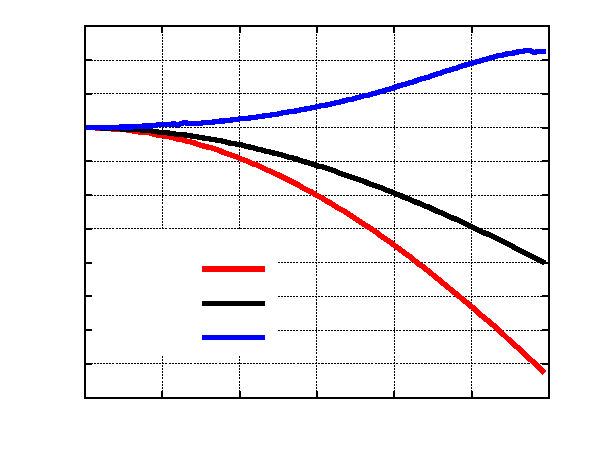
\includegraphics{IsopointSimulationPolydispersity}}%
    \gplfronttext
  \end{picture}%
\endgroup
}\label{fig:IsopointSimulationPolydispersity}}
		\subfloat[Electron density reange]{\resizebox{0.44\linewidth}{!}{% GNUPLOT: LaTeX picture with Postscript
\begingroup
  \makeatletter
  \providecommand\color[2][]{%
    \GenericError{(gnuplot) \space\space\space\@spaces}{%
      Package color not loaded in conjunction with
      terminal option `colourtext'%
    }{See the gnuplot documentation for explanation.%
    }{Either use 'blacktext' in gnuplot or load the package
      color.sty in LaTeX.}%
    \renewcommand\color[2][]{}%
  }%
  \providecommand\includegraphics[2][]{%
    \GenericError{(gnuplot) \space\space\space\@spaces}{%
      Package graphicx or graphics not loaded%
    }{See the gnuplot documentation for explanation.%
    }{The gnuplot epslatex terminal needs graphicx.sty or graphics.sty.}%
    \renewcommand\includegraphics[2][]{}%
  }%
  \providecommand\rotatebox[2]{#2}%
  \@ifundefined{ifGPcolor}{%
    \newif\ifGPcolor
    \GPcolortrue
  }{}%
  \@ifundefined{ifGPblacktext}{%
    \newif\ifGPblacktext
    \GPblacktextfalse
  }{}%
  % define a \g@addto@macro without @ in the name:
  \let\gplgaddtomacro\g@addto@macro
  % define empty templates for all commands taking text:
  \gdef\gplbacktext{}%
  \gdef\gplfronttext{}%
  \makeatother
  \ifGPblacktext
    % no textcolor at all
    \def\colorrgb#1{}%
    \def\colorgray#1{}%
  \else
    % gray or color?
    \ifGPcolor
      \def\colorrgb#1{\color[rgb]{#1}}%
      \def\colorgray#1{\color[gray]{#1}}%
      \expandafter\def\csname LTw\endcsname{\color{white}}%
      \expandafter\def\csname LTb\endcsname{\color{black}}%
      \expandafter\def\csname LTa\endcsname{\color{black}}%
      \expandafter\def\csname LT0\endcsname{\color[rgb]{1,0,0}}%
      \expandafter\def\csname LT1\endcsname{\color[rgb]{0,1,0}}%
      \expandafter\def\csname LT2\endcsname{\color[rgb]{0,0,1}}%
      \expandafter\def\csname LT3\endcsname{\color[rgb]{1,0,1}}%
      \expandafter\def\csname LT4\endcsname{\color[rgb]{0,1,1}}%
      \expandafter\def\csname LT5\endcsname{\color[rgb]{1,1,0}}%
      \expandafter\def\csname LT6\endcsname{\color[rgb]{0,0,0}}%
      \expandafter\def\csname LT7\endcsname{\color[rgb]{1,0.3,0}}%
      \expandafter\def\csname LT8\endcsname{\color[rgb]{0.5,0.5,0.5}}%
    \else
      % gray
      \def\colorrgb#1{\color{black}}%
      \def\colorgray#1{\color[gray]{#1}}%
      \expandafter\def\csname LTw\endcsname{\color{white}}%
      \expandafter\def\csname LTb\endcsname{\color{black}}%
      \expandafter\def\csname LTa\endcsname{\color{black}}%
      \expandafter\def\csname LT0\endcsname{\color{black}}%
      \expandafter\def\csname LT1\endcsname{\color{black}}%
      \expandafter\def\csname LT2\endcsname{\color{black}}%
      \expandafter\def\csname LT3\endcsname{\color{black}}%
      \expandafter\def\csname LT4\endcsname{\color{black}}%
      \expandafter\def\csname LT5\endcsname{\color{black}}%
      \expandafter\def\csname LT6\endcsname{\color{black}}%
      \expandafter\def\csname LT7\endcsname{\color{black}}%
      \expandafter\def\csname LT8\endcsname{\color{black}}%
    \fi
  \fi
  \setlength{\unitlength}{0.0500bp}%
  \begin{picture}(5668.00,4534.00)%
    \gplgaddtomacro\gplbacktext{%
      \csname LTb\endcsname%
      \put(946,1014){\makebox(0,0)[r]{\strut{}-0.5}}%
      \csname LTb\endcsname%
      \put(946,1789){\makebox(0,0)[r]{\strut{} 0}}%
      \csname LTb\endcsname%
      \put(946,2564){\makebox(0,0)[r]{\strut{} 0.5}}%
      \csname LTb\endcsname%
      \put(946,3339){\makebox(0,0)[r]{\strut{} 1}}%
      \csname LTb\endcsname%
      \put(946,4114){\makebox(0,0)[r]{\strut{} 1.5}}%
      \csname LTb\endcsname%
      \put(1078,484){\makebox(0,0){\strut{} 330}}%
      \csname LTb\endcsname%
      \put(1677,484){\makebox(0,0){\strut{} 340}}%
      \csname LTb\endcsname%
      \put(2276,484){\makebox(0,0){\strut{} 350}}%
      \csname LTb\endcsname%
      \put(2875,484){\makebox(0,0){\strut{} 360}}%
      \csname LTb\endcsname%
      \put(3474,484){\makebox(0,0){\strut{} 370}}%
      \csname LTb\endcsname%
      \put(4073,484){\makebox(0,0){\strut{} 380}}%
      \csname LTb\endcsname%
      \put(4672,484){\makebox(0,0){\strut{} 390}}%
      \csname LTb\endcsname%
      \put(5271,484){\makebox(0,0){\strut{} 400}}%
      \put(176,2486){\rotatebox{-270}{\makebox(0,0){\strut{}Deviation / $\%$}}}%
      \put(3174,154){\makebox(0,0){\strut{}$\rho_{max}$ / nm$^{-3}$}}%
    }%
    \gplgaddtomacro\gplfronttext{%
    }%
    \gplbacktext
    \put(0,0){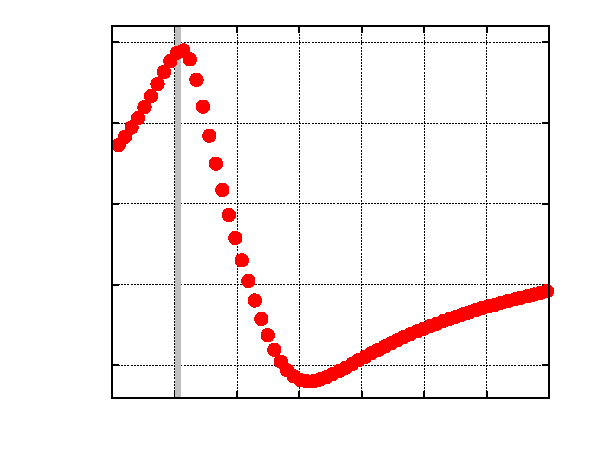
\includegraphics{IsopointSimulationRange}}%
    \gplfronttext
  \end{picture}%
\endgroup
}\label{fig:IsopointSimulationRange}}

	\caption{Deviation of the size calculated from $q_1^{\star}$ from the nominal value depending on a) the contrast range (330 nm$^{-3}$, $\rho_{\text{max}}$) or b) the polydispersity of the core-shell particle.}

\end{figure}

Besides, this work demonstrates that the $q^{\star}$ value determined with the previously described method depends on the range of solvent densities used in the contrast variation experiment. For this purpose, it was simulated the result of a contrast variation experiment with 10 different solvent densities for a polymeric particle with the morphology and size distribution obtained with the core-shell model in section \ref{sec:size_validation}. Using a lower bound to the contrast range of $\rho_{\text{min}}=330$ nm$^{-3}$ and increasing systematically the upper limit, it is shown in figure \ref{fig:IsopointSimulationRange} that the calculated result deviates from the nominal value up to 1.5$\%$. 

In this example, the largest deviations occur when the contrast range excludes the average density of the latex, e.g. match point (depicted as a vertical line in figure \ref{fig:IsopointSimulationRange}), or when $\rho_{\text{max}}$ is close to this matching density. This observation conflicts partly with the initial intuition that this technique is independent of the experimental proceeding, although the method can avoid this problem by selecting the solvent electron density range skillfully i.e. equidistantly distributed around the match point. This could be one explanation behind the size differences observed in figure \ref{fig:PSPlainSizeComparison} between the SAXS results.

The isoscattering point approach to contrast variation SAXS data evaluation presents certain assets which can not be ignored. For instance, the independence of $q^{\star}$ from the sample contrast facilitates its easy application, although the solvent electron density range must be chosen with care and always around the average electron density of the particle. On the other hand, the diffuseness of the isoscattering point position due to the polydispersity and ellipticity of the sample arises as an indisputable drawback.

\section{Determination of the particle physical density}
\label{sec:physical_density}
In contrast variation SAXS, the solvent electron density which matches the average electron density of the particle ($\rho_0$) corresponds to a minimum in the intensity of the scattering curve. In order to quantify the particle density, the scattering intensity of PS-Plain at zero angle $I(0)$ is examined along the contrast range of the experiment as shown in figure \ref{fig:PSPlainAverageDensity}. The value of $I(0)$ was determined by extrapolation to $q\rightarrow 0$ using a spherical form factor function fitted to the available range before the first minimum.

\begin{figure}
	\begin{center}
		% GNUPLOT: LaTeX picture with Postscript
\begingroup
  \makeatletter
  \providecommand\color[2][]{%
    \GenericError{(gnuplot) \space\space\space\@spaces}{%
      Package color not loaded in conjunction with
      terminal option `colourtext'%
    }{See the gnuplot documentation for explanation.%
    }{Either use 'blacktext' in gnuplot or load the package
      color.sty in LaTeX.}%
    \renewcommand\color[2][]{}%
  }%
  \providecommand\includegraphics[2][]{%
    \GenericError{(gnuplot) \space\space\space\@spaces}{%
      Package graphicx or graphics not loaded%
    }{See the gnuplot documentation for explanation.%
    }{The gnuplot epslatex terminal needs graphicx.sty or graphics.sty.}%
    \renewcommand\includegraphics[2][]{}%
  }%
  \providecommand\rotatebox[2]{#2}%
  \@ifundefined{ifGPcolor}{%
    \newif\ifGPcolor
    \GPcolortrue
  }{}%
  \@ifundefined{ifGPblacktext}{%
    \newif\ifGPblacktext
    \GPblacktextfalse
  }{}%
  % define a \g@addto@macro without @ in the name:
  \let\gplgaddtomacro\g@addto@macro
  % define empty templates for all commands taking text:
  \gdef\gplbacktext{}%
  \gdef\gplfronttext{}%
  \makeatother
  \ifGPblacktext
    % no textcolor at all
    \def\colorrgb#1{}%
    \def\colorgray#1{}%
  \else
    % gray or color?
    \ifGPcolor
      \def\colorrgb#1{\color[rgb]{#1}}%
      \def\colorgray#1{\color[gray]{#1}}%
      \expandafter\def\csname LTw\endcsname{\color{white}}%
      \expandafter\def\csname LTb\endcsname{\color{black}}%
      \expandafter\def\csname LTa\endcsname{\color{black}}%
      \expandafter\def\csname LT0\endcsname{\color[rgb]{1,0,0}}%
      \expandafter\def\csname LT1\endcsname{\color[rgb]{0,1,0}}%
      \expandafter\def\csname LT2\endcsname{\color[rgb]{0,0,1}}%
      \expandafter\def\csname LT3\endcsname{\color[rgb]{1,0,1}}%
      \expandafter\def\csname LT4\endcsname{\color[rgb]{0,1,1}}%
      \expandafter\def\csname LT5\endcsname{\color[rgb]{1,1,0}}%
      \expandafter\def\csname LT6\endcsname{\color[rgb]{0,0,0}}%
      \expandafter\def\csname LT7\endcsname{\color[rgb]{1,0.3,0}}%
      \expandafter\def\csname LT8\endcsname{\color[rgb]{0.5,0.5,0.5}}%
    \else
      % gray
      \def\colorrgb#1{\color{black}}%
      \def\colorgray#1{\color[gray]{#1}}%
      \expandafter\def\csname LTw\endcsname{\color{white}}%
      \expandafter\def\csname LTb\endcsname{\color{black}}%
      \expandafter\def\csname LTa\endcsname{\color{black}}%
      \expandafter\def\csname LT0\endcsname{\color{black}}%
      \expandafter\def\csname LT1\endcsname{\color{black}}%
      \expandafter\def\csname LT2\endcsname{\color{black}}%
      \expandafter\def\csname LT3\endcsname{\color{black}}%
      \expandafter\def\csname LT4\endcsname{\color{black}}%
      \expandafter\def\csname LT5\endcsname{\color{black}}%
      \expandafter\def\csname LT6\endcsname{\color{black}}%
      \expandafter\def\csname LT7\endcsname{\color{black}}%
      \expandafter\def\csname LT8\endcsname{\color{black}}%
    \fi
  \fi
  \setlength{\unitlength}{0.0500bp}%
  \begin{picture}(5668.00,4534.00)%
    \gplgaddtomacro\gplbacktext{%
      \csname LTb\endcsname%
      \put(616,768){\makebox(0,0)[r]{\strut{} 0}}%
      \csname LTb\endcsname%
      \put(616,1404){\makebox(0,0)[r]{\strut{} 2}}%
      \csname LTb\endcsname%
      \put(616,2041){\makebox(0,0)[r]{\strut{} 4}}%
      \csname LTb\endcsname%
      \put(616,2677){\makebox(0,0)[r]{\strut{} 6}}%
      \csname LTb\endcsname%
      \put(616,3314){\makebox(0,0)[r]{\strut{} 8}}%
      \csname LTb\endcsname%
      \put(616,3951){\makebox(0,0)[r]{\strut{} 10}}%
      \csname LTb\endcsname%
      \put(748,484){\makebox(0,0){\strut{} 334}}%
      \csname LTb\endcsname%
      \put(1570,484){\makebox(0,0){\strut{} 336}}%
      \csname LTb\endcsname%
      \put(2393,484){\makebox(0,0){\strut{} 338}}%
      \csname LTb\endcsname%
      \put(3215,484){\makebox(0,0){\strut{} 340}}%
      \csname LTb\endcsname%
      \put(4037,484){\makebox(0,0){\strut{} 342}}%
      \csname LTb\endcsname%
      \put(4860,484){\makebox(0,0){\strut{} 344}}%
      \put(176,2486){\rotatebox{-270}{\makebox(0,0){\strut{}$I(0)$ / a.u.}}}%
      \put(3009,154){\makebox(0,0){\strut{}Solvent Electron density / nm$^{-3}$}}%
    }%
    \gplgaddtomacro\gplfronttext{%
    }%
    \gplbacktext
    \put(0,0){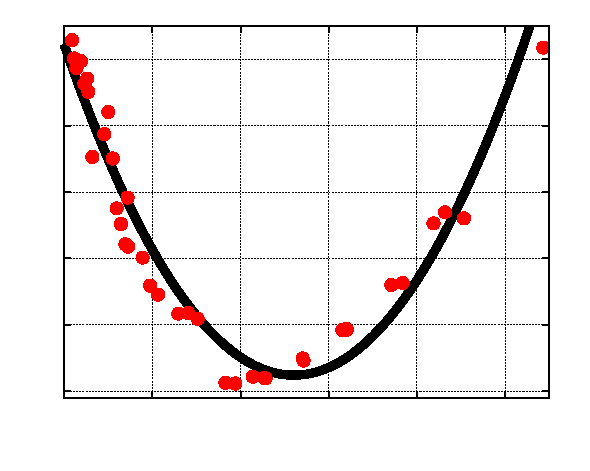
\includegraphics{PSPlainAverageDensity}}%
    \gplfronttext
  \end{picture}%
\endgroup

	\end{center}
	\caption{Intensity at zero-angle of PS-Plain particles as a function of the solvent electron density measured with continuous contrast variation in SAXS. The minimum defines the average electron density of the particle.}
	\label{fig:PSPlainAverageDensity}
\end{figure}

This parameter behaves parabollically around the average electron density of the particle like $I(0)\propto \left( \rho_0 - \rho_{solv} \right)^2$\citep{avdeev_contrast_2007}. From the position of the minimum, $\rho_0$ can thus be solved. The parabolic fit to the data is plotted as a black line in figure \ref{fig:PSPlainAverageDensity} and results in $\rho_0=\left(339.2\pm1.0\right)$ nm$^{-3}$, which is consistent with the tabulated value of dry bulk polystyrene 339.7 nm$^{-3}$\citep{dingenouts_analysis_1999}.

The electron density is directly proportional to the physical density. Nevertheless, an assumption about the polymer (or monomer) components and their atomic structure is necessary for the calculation.Therefore, a typical value of $Z/A=0.54$ was adopted, where $Z$ and $A$ are the average atomic number and mass of the polymer respectively.

\subsection{Validation through comparison with DCS}

In figure \ref{fig:DensityComparison}, the value of ($1.043\pm0.003$) g cm$^{-3}$ obtained with the $I(0)$ approach from the continuous contrast variation experiment is compared to the average density of the PS-Plain colloid measured with different DCS configurations. For single disc setups, the size value used for the density calculation was 147 nm, as measured by SAXS, while combining the information from the two setups allowed the measurement of the density independently of the particle diameter, as explained in $\S$\ref{sec:size_validation}.

The results agree with each other within their stated measurement uncertainties, although DCS measurements exhibit slightly higher densities than SAXS. Typical causes of systematic errors in DCS are the inaccuracy of the size and density of the calibration standard and the thermal variation in the centrifuge gradient during the measurements, which affect its viscosity and density\citep{kamiti_simultaneous_2012}. A temperature variation within the gradient of about 7 degree C before and after measurements was detected and a period of 30 min was considered appropriate to reach reliable thermal equilibrium. In the low density disc configuration, the accuracy of the average density of the D$_2$0 sucrose gradient becomes an important source of uncertainty.
\begin{figure}
	\begin{center}
		% GNUPLOT: LaTeX picture with Postscript
\begingroup
  \makeatletter
  \providecommand\color[2][]{%
    \GenericError{(gnuplot) \space\space\space\@spaces}{%
      Package color not loaded in conjunction with
      terminal option `colourtext'%
    }{See the gnuplot documentation for explanation.%
    }{Either use 'blacktext' in gnuplot or load the package
      color.sty in LaTeX.}%
    \renewcommand\color[2][]{}%
  }%
  \providecommand\includegraphics[2][]{%
    \GenericError{(gnuplot) \space\space\space\@spaces}{%
      Package graphicx or graphics not loaded%
    }{See the gnuplot documentation for explanation.%
    }{The gnuplot epslatex terminal needs graphicx.sty or graphics.sty.}%
    \renewcommand\includegraphics[2][]{}%
  }%
  \providecommand\rotatebox[2]{#2}%
  \@ifundefined{ifGPcolor}{%
    \newif\ifGPcolor
    \GPcolortrue
  }{}%
  \@ifundefined{ifGPblacktext}{%
    \newif\ifGPblacktext
    \GPblacktextfalse
  }{}%
  % define a \g@addto@macro without @ in the name:
  \let\gplgaddtomacro\g@addto@macro
  % define empty templates for all commands taking text:
  \gdef\gplbacktext{}%
  \gdef\gplfronttext{}%
  \makeatother
  \ifGPblacktext
    % no textcolor at all
    \def\colorrgb#1{}%
    \def\colorgray#1{}%
  \else
    % gray or color?
    \ifGPcolor
      \def\colorrgb#1{\color[rgb]{#1}}%
      \def\colorgray#1{\color[gray]{#1}}%
      \expandafter\def\csname LTw\endcsname{\color{white}}%
      \expandafter\def\csname LTb\endcsname{\color{black}}%
      \expandafter\def\csname LTa\endcsname{\color{black}}%
      \expandafter\def\csname LT0\endcsname{\color[rgb]{1,0,0}}%
      \expandafter\def\csname LT1\endcsname{\color[rgb]{0,1,0}}%
      \expandafter\def\csname LT2\endcsname{\color[rgb]{0,0,1}}%
      \expandafter\def\csname LT3\endcsname{\color[rgb]{1,0,1}}%
      \expandafter\def\csname LT4\endcsname{\color[rgb]{0,1,1}}%
      \expandafter\def\csname LT5\endcsname{\color[rgb]{1,1,0}}%
      \expandafter\def\csname LT6\endcsname{\color[rgb]{0,0,0}}%
      \expandafter\def\csname LT7\endcsname{\color[rgb]{1,0.3,0}}%
      \expandafter\def\csname LT8\endcsname{\color[rgb]{0.5,0.5,0.5}}%
    \else
      % gray
      \def\colorrgb#1{\color{black}}%
      \def\colorgray#1{\color[gray]{#1}}%
      \expandafter\def\csname LTw\endcsname{\color{white}}%
      \expandafter\def\csname LTb\endcsname{\color{black}}%
      \expandafter\def\csname LTa\endcsname{\color{black}}%
      \expandafter\def\csname LT0\endcsname{\color{black}}%
      \expandafter\def\csname LT1\endcsname{\color{black}}%
      \expandafter\def\csname LT2\endcsname{\color{black}}%
      \expandafter\def\csname LT3\endcsname{\color{black}}%
      \expandafter\def\csname LT4\endcsname{\color{black}}%
      \expandafter\def\csname LT5\endcsname{\color{black}}%
      \expandafter\def\csname LT6\endcsname{\color{black}}%
      \expandafter\def\csname LT7\endcsname{\color{black}}%
      \expandafter\def\csname LT8\endcsname{\color{black}}%
    \fi
  \fi
  \setlength{\unitlength}{0.0500bp}%
  \begin{picture}(5668.00,4534.00)%
    \gplgaddtomacro\gplbacktext{%
      \csname LTb\endcsname%
      \put(548,1409){\makebox(0,0)[r]{\strut{} 1.04}}%
      \csname LTb\endcsname%
      \put(548,1779){\makebox(0,0)[r]{\strut{} 1.05}}%
      \csname LTb\endcsname%
      \put(548,2150){\makebox(0,0)[r]{\strut{} 1.06}}%
      \csname LTb\endcsname%
      \put(548,2520){\makebox(0,0)[r]{\strut{} 1.07}}%
      \csname LTb\endcsname%
      \put(868,1092){\rotatebox{-45}{\makebox(0,0)[l]{\strut{}Normal Disc}}}%
      \csname LTb\endcsname%
      \put(1338,1092){\rotatebox{-45}{\makebox(0,0)[l]{\strut{}Combined}}}%
      \csname LTb\endcsname%
      \put(1809,1092){\rotatebox{-45}{\makebox(0,0)[l]{\strut{}Low Density}}}%
      \csname LTb\endcsname%
      \put(2279,1092){\rotatebox{-45}{\makebox(0,0)[l]{\strut{}SAXS}}}%
      \csname LTb\endcsname%
      \put(3220,1092){\rotatebox{-45}{\makebox(0,0)[l]{\strut{}DCS}}}%
      \csname LTb\endcsname%
      \put(3690,1092){\rotatebox{-45}{\makebox(0,0)[l]{\strut{}SAXS}}}%
      \csname LTb\endcsname%
      \put(4631,1092){\rotatebox{-45}{\makebox(0,0)[l]{\strut{}DCS}}}%
      \csname LTb\endcsname%
      \put(5101,1092){\rotatebox{-45}{\makebox(0,0)[l]{\strut{}SAXS}}}%
      \put(-222,2680){\rotatebox{-270}{\makebox(0,0){\strut{}Density / g cm$^{-3}$}}}%
    }%
    \gplgaddtomacro\gplfronttext{%
    }%
    \gplgaddtomacro\gplbacktext{%
      \csname LTb\endcsname%
      \put(548,3349){\makebox(0,0)[r]{\strut{} 1.17}}%
      \csname LTb\endcsname%
      \put(548,3846){\makebox(0,0)[r]{\strut{} 1.18}}%
      \colorrgb{0.00,0.00,1.00}%
      \put(1235,2952){\makebox(0,0)[l]{\strut{}\smaller PS-Plain}}%
      \put(3032,3051){\makebox(0,0)[l]{\strut{}\smaller PS-COOH}}%
      \put(4066,4243){\makebox(0,0)[l]{\strut{}\smaller PMMA-COOH}}%
    }%
    \gplgaddtomacro\gplfronttext{%
    }%
    \gplbacktext
    \put(0,0){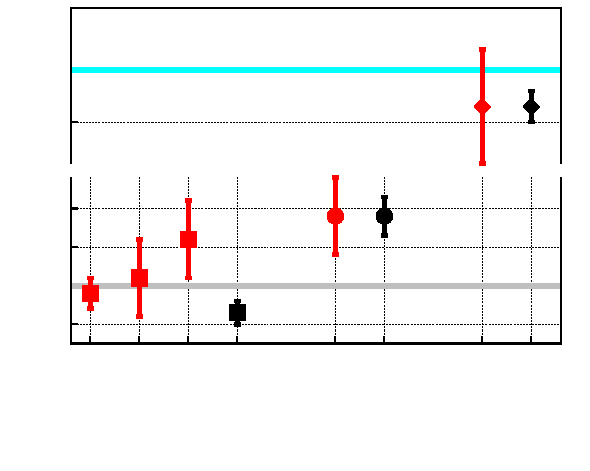
\includegraphics{DensityComparison}}%
    \gplfronttext
  \end{picture}%
\endgroup

	\end{center}
	\caption{Comparison between the physical densities of 3 polymeric colloids measured with SAXS using the $I(0)$ approach and DCS: PS-Plain (squares), PS-COOH (circles) and PMMA-COOH (diamonds). The nominal densities of polystyrene (1.05 g cm$^-3$) and PMMA (1.18 g cm$^-3$) are also shown in the plot as horizontal lines [22].}
	\label{fig:DensityComparison}
\end{figure}
\subsubsection{Uncertainties}
In SAXS, the uncertainty is associated to the vertical size of the focused X-ray beam as in \citep{garcia-diez_nanoparticle_2015}. Furthermore, the result can be affected by the polymeric composition of the colloid, and therefore, the assumption of $Z/A$..

\subsection{Use for heavier polymeric colloids}
The applicability of the continuous contrast variation techniques is further discussed by comparing with DCS for higher-density polymeric colloids, as summarized in figure \ref{fig:DensityComparison}. The density of the PS-COOH particles derived from the $I(0)$ approach is in excellent agreement with that measured by DCS using a standard configuration and assuming a particle diameter of 99.4 nm, which was obtained by SAXS. Considering the similar electronic composition of these polymers and the average electron density of the particle $\rho_0=346$ nm\(^{-3}\), an average physical density of the particles of $\rho=1.07$ g/cm\(^{3}\) can be calculated. These core-shell particles, more dense than polystyrene as detailed in section \ref{sec:coreshell_fit}, illustrate the tendency during the emulsion polymerization to segregate polar and nonpolar components \citep{dingenouts_structure_1994}.

Similarly, the density of the PMMA-COOH colloids was measured using the standard DCS setup and assuming a diameter of 186.5 nm, as measured by SAXS. This value is compared to the density obtained by computing the intensity at zero-angle of a continuous contrast variation experiment. Again, both techniques are in excellent agreement and reveal a physical density slightly lower than the expected PMMA density of 1.18 g cm$^{-3}$\citep{dingenouts_analysis_1999}.

This result highlights the fact that the density of polymeric colloids in suspension may vary from that of bulk materials, for example dry particles. For instance, a volume variation can be expected when going from the MMA monomer to the polymer PMMA\citep{nichols_prediction_1950} which might reduce the colloid density.

\section{Summary}
This work demonstrates how continuous contrast variation in SAXS emerges as a powerful characterisation technique for polymeric colloids, which can determine their size and density in a traceable way. For instance, the accuracy in the density information achieved with the density gradient technique is remarkable and extends along a rather large density range of polymers.

Since contrast variation in SAXS is very sensitive to small electron density differences in the colloid morphology, the applicability of this method to investigate the inner structure of 3 different particles has been discussed. This is of paramount importance in polymeric particle characterisation because the direct observation by imaging techniques is inadequate for this purpose.

The detection of core-shell structures in polymeric colloids appears as essential for understanding the possible processes occurring during the particle formation, e.g. the consequences of emulsion polymerization synthesis. 

These results were compared successfully with other techniques. In particular, SAXS measurements of the density of these colloids are in excellent agreement with those performed by DCS. The use of a novel DCS setup is also shown, which makes use of a centrifuge disc where the colloids float through a gradient of higher density, in contrast to a standard setup where the particles typically sediment. The use of the two complementary DCS configurations allowed the simultaneous determination of both the size and density of polymeric colloids consistently with the SAXS results.

Furthermore, different evaluation approaches to contrast variation SAXS data are examined in detail. The isoscattering point framework is found to be of easy utilization and very appropriate for spherical and quite monodisperse colloids. On the other hand, the calculation of the scattering shape factor arises as a precise sizing technique which can additionally provide an insight into the particle shape, although a high number of measurements with different contrasts and an accurate calibration of the system are required.

With the continuous contrast variation technique in SAXS, a more precise characterisation of the morphology of polymeric particles is achieved which opens new opportunities to investigate complex polymeric colloids. Besides, both ensemble techniques presented in this paper arise as powerful methods which can describe simultaneously the density and size distribution of polymeric colloids at the nanoscale.
